% DO NOT COMPILE THIS FILE DIRECTLY!
% This is included by the other .tex files.

\begin{frame}[t,plain]
\titlepage
\end{frame}

\begin{frame}{Outline}
	\tableofcontents
\end{frame}

%============================================================================
\section{Preliminaries}
%============================================================================

\subsection{Distributions}

\begin{frame}{Distributions}

\begin{itemize}\itemsep1em
	\item $\Omega\subset\R^d$ open and bounded set.
	\item $\D(\Omega)=\{\varphi\in\mathcal{C}^\infty(\Omega)\colon\varphi\text{ tiene soporte compacto en }\Omega\}$. 
	
	\item \structure{\textbf{Space of distributions}}: $\D'(\Omega)$ (dual space)
	\begin{itemize}\itemsep1em
		\item $L^p(\Omega)\hookrightarrow\D '(\Omega)$ defined for every $v\in L^p(\Omega)$ as $\alert{\dualD{v}{\varphi}}=v(\varphi)\coloneqq\int_\Omega v \varphi$, $\forall \varphi\in\D(\Omega)$;
	\end{itemize}

	\item Let $v\in L^p(\Omega)$, if $g_\alpha=\partial^\alpha v=D^\alpha v\in L^p(\Omega)$ verifies $\dualD{D^\alpha v}{\varphi}=(-1)^{\left|\alpha\right|}\int_\Omega v D^\alpha \varphi$ for every $\varphi\in\D(\Omega)$ then $g_\alpha$ is named \structure{\textbf{weak derivative}}.

\end{itemize}
\end{frame}

\subsection{Sobolev spaces}
\begin{frame}{Sobolev spaces}
Assume that $m\in\N\cup\left\{0\right\}$ and $1\leq p\leq+\infty$, $p\in\N$.
\begin{itemize}\itemsep1em
	\item$\displaystyle\alert{W^{m,p}(\Omega)}\coloneqq\{v\in L^p(\Omega):\forall\alpha\in\N^d\mbox{ con }\left|\alpha\right|\leq m, \partial^\alpha v\in L^p(\Omega)\}$
	\begin{itemize}\itemsep1em
		\item For $p=2$, $\alert{H^{m}(\Omega)}\coloneqq W^{m,2}(\Omega).$
	\end{itemize}
	
	\item Norms defined $\forall v\in W^{m,p}(\Omega)$:
	\begin{itemize}\itemsep1em
		\item $\displaystyle \alert{\|v\|_{W^{m,p}(\Omega)}}\coloneqq\left(\suma{\substack{\alpha\in\N^d \\ \left|\alpha\right|\leq m}}{}\|\partial^\alpha v\|^p_{L^p(\Omega)}\right)^{1/p}\text{ si }p<+\infty$,
		\item $\displaystyle \alert{\|v\|_{W^{m,\infty}(\Omega)}}\coloneqq\max_{\substack{\alpha\in\N^d \\ \left|\alpha\right|\leq m}}{}\|\partial^\alpha v\|_{L^\infty(\Omega)}\text{ si }p=+\infty$.
	\end{itemize}
	
	\item $\alert{H_0^1(\Omega)}\coloneqq\left\{v\in H^1(\Omega):v_{|_{\partial\Omega}}\equiv 0\right\}$;
	\item $\alert{H(\text{div};\Omega)}\coloneqq\left\{\tau\in(L^2(\Omega))^d\colon\nabla\cdot\tau\in L^2(\Omega) \right\}.$
	
\end{itemize}

\end{frame}

\begin{frame}{Trace}

	\begin{theorem}[Trace]
		
		The trace mapping
		\begin{align*}
		\alert{\gamma}\colon H^1(\Omega)\cap\mathcal{C}^0(\bar{\Omega})&\to L^2(\partial\Omega)\cap \mathcal{C}(\bar{\partial\Omega})\\
		v	&\mapsto\alert{\gamma(v)}\coloneqq v_{|_{\partial\Omega}}.
		\end{align*}
		is extended by continuity to a continuous linear mapping of $H^1(\Omega)$ into $L^2(\partial\Omega)$,  again called $\gamma$.
		
		There is $C>0$ such that $\forall v\in H^1(\Omega)$ it is $$\norma{\gamma(v)}_{L^2(\partial \Omega)}\leq C\norma{v}_{H^1(\Omega)}.$$
	\end{theorem}
	%\pause
	% \textbf{Remark}: extends integration by parts formula to functions of $H^1(\Omega)$.
	
\end{frame}

\subsection{Variational formulation}

\begin{frame}{Linear PDE of order 2}
\begin{block}{}
\begin{equation*}
\label{ecuacion_general}
\left\{
\begin{aligned}
\mathcal{L}u&=f & \text{en } &\Omega, \\
\mathcal{B}u&=g & \text{en } &\partial\Omega,
\end{aligned}
\right.
\end{equation*}
\end{block}

\begin{itemize}\itemsep1em
\item $\Omega\subset \R^d$ a regular enough open and bounded set (for instance, a polygonal domain).
\item Differential operator $\mathcal{L}$ defined for every $u\colon\Omega\to\R$ as $$\mathcal{L}u=-\nabla\cdot(a\nabla u)+b\nabla u+c u$$ with $a\in [L^\infty(\Omega)]^{d,d}$, $\mathbf{b}\in [L^\infty(\Omega)]^d$ y $c\in L^\infty(\Omega)$.
\item $f\in L^2(\Omega)$.
\item Boundary condition operator $\mathcal{B}$.
\item $g\colon\Omega\to\R$.
\end{itemize}

\end{frame}

\begin{frame}{Integration by parts formula}
	\begin{theorem}[Integration by parts formula]
		
		Let $u, v\in \mathcal{C}^1(\bar\Omega)$, they satisfy
		\begin{equation*}
		\label{formula_int_por_partes}
		\int_\Omega u(x)\frac{\partial v}{\partial x_i}(x)dx=-\int_\Omega v(x)\frac{\partial u}{\partial x_i}(x)dx+\int_{\partial \Omega}u(x)v(x)\mathbf{n}_i(x)ds.
		\end{equation*}
		
	\end{theorem}
	
\end{frame}

\begin{frame}{Variational problem}

\begin{enumerate}
	\item Defined the solution space $\S\subseteq H^1(\Omega)$  regular enough (in the weak sense).
	\item \structure{\textbf{Formulación variacional}}: find a function $u\in \S$ that verifies $$a(u,v)=L(v)\text{ for every }v\in \S.$$
		\begin{itemize}\itemsep1em
			\item $a\colon\S\times\S\to\R$ bilinear form; 
			\item $L\colon\S\to\R$ linear form.
		\end{itemize}
\end{enumerate}

\end{frame}

\begin{frame}{Properties of bilinear form}
	\begin{definicion}
		Let $V$ a Hilbert space and let $a(\cdot,\cdot):V\times V\longrightarrow\R$ a bilinear form. Then, $a(\cdot,\cdot)$ is
		\begin{itemize}
			\item \structure{\textbf{continuous}} if there is $M>0$ such that $$a(v,w)\geq\nu\norma{v}\norma{w}\text{ for every } v,w\in V.$$
			\item \structure{\textbf{coercive}} if there is $\nu>0$ such that $$a(v,v)\geq\nu\norma{v}^2\text{ for every } v\in V.$$
		\end{itemize}
	\end{definicion}
\end{frame}

\begin{frame}{Lax-Milgram Theorem}

\begin{theorem}[Lax-Milgram]
	\label{theorem:Lax_Milgram}
	Let $V$ be a real Hilbert space, $L(\cdot)$ continuous linear form in $V$ y $a(\cdot,\cdot)$ a coercive (with coercivity constant $\alpha$) and continuous bilinear form in $V$. The variational formulation $$a(u,v)=L(v)\text{ for every }v\in V$$ have a unique solution $u\in V$ which depends continuously on the linear form $L$ as follows
	$$\norma{u}_V\le \frac{1}{\alpha}\norma{L}_{V'}.$$
\end{theorem}

\end{frame}

%-------------------------------
\section{Finite Element Method}
%-------------------------------

\subsection{Elliptic problem}

\begin{frame}{Elliptic problem}
Consider the Poisson problem:
\begin{block}{}
\begin{equation*}
\left\{
\begin{aligned}
-\Delta u&=f & \text{en } &\Omega, \\
u&=0 & \text{en } &\partial\Omega,
\end{aligned}
\right.
\end{equation*}
\end{block}
where $f\in L^2\left(\Omega\right)$.
\end{frame}

% \subsection{Formulación variacional continua}

\begin{frame}[allowframebreaks]{Continuous variational formulation}

\textbf{Space of solutions}: $\alert{H_0^1(\Omega)}$.
\begin{itemize}\itemsep1em
	\item $a\colon H^1_0(\Omega)\times H_0^1(\Omega)\to\R$, $\displaystyle \alert{a(u,v)}\coloneqq\int_\Omega\nabla u\nabla v$;
	\item $L\colon H_0^1(\Omega)\to\R$, $\displaystyle \alert{L(v)}\coloneqq\int_\Omega f v$.
\end{itemize}
\textbf{Variational problem}:
\begin{block}{}
	\begin{center}
	$\text{find } u\in H^1_0(\Omega) \text{ such that } a(u,v)=L(v)\text{ for every } v\in H_0^1(\Omega)$.
	\end{center}
\end{block}
\framebreak
\begin{theorem}
	The bilinear form $a(\cdot,\cdot)$ is coercive and continuous.
\end{theorem}

\begin{itemize}\itemsep1em
	\item The model problem and its weak variational formulation are \alert{equivalent}.
	\begin{itemize}\itemsep1em
		\item If $u\in H^2(\Omega)$ is a solution of the model problem $\Rightarrow$ it is a solution of the variational problem.
		\item If $u\in H_0^1(\Omega)$ is solution of the variational problem $\Rightarrow$ it is solution of the model problem.
	\end{itemize}
	\item \alert{Lax-Milgram} $\Rightarrow$ there is a unique solution.
\end{itemize}

\end{frame}

\subsubsection{Numerical approximation}

\begin{frame}{Galerkin method}
	\begin{block}{}
	\begin{center}
	Choose $\alert{V_h\subseteq V}$ finite-dimensional with a basis $\left\{\varphi_i\right\}_{i\in\left\{1,2,\ldots,N_h \right\}}$
	\end{center}
	\end{block}
	
	\vspace*{-0.3cm}
	\begin{itemize}
	\item Find $u\in V$ such that $a(u,v)=L(v)$ for every $v\in V$.
	\end{itemize}
	\vspace*{0.1cm}
	$$\Big{\downarrow}$$
	\vspace*{-0.3cm}
	\begin{itemize}
	\item Choose $u_h\in V_h$ such that $a(u_h,v_h)=L(v_h)$ for every $v_h\in V_h$.
	\end{itemize}
	\vspace*{0.1cm}
	$$\Big{\Updownarrow}$$
	\vspace*{-0.3cm}
	\begin{itemize}
	\item Solve the linear system $A\mathbf{U}=\mathbf{F}$ where:
	\vspace*{0.3cm}
	\begin{itemize}
		\item $A=\left(A_{i j}\right)_{i, j\in\left\{1,2,\ldots,N_h\right\}}$ with $A_{i j}=a(\varphi_j,\varphi_i)$;
		\item $\mathbf{U}=\left(U_1,U_2,\ldots,U_{N_h}\right)^t$ with $u_h=\displaystyle\sum_{i=1}^{N_h}U_i\varphi_i$;
		\item $\mathbf{F}=\left(F_1,F_2,\ldots,F_{N_h}\right)^t$ with $F_i=L\left(\varphi_i\right)$.
	\end{itemize}
	\end{itemize}
\end{frame}
	
% \begin{frame}{Cota de error}
% 	\begin{lemma}
% 		Supongamos que $a(\cdot,\cdot)$ es coercitiva y continua. Se verifica que
% 		\begin{equation*}
% 		\norma{u-u_h}\leq \frac{M}{\nu} \inf_{v_h\in V_h}\norma{u-v_h}
% 		\end{equation*}
% 		donde $M>0$ y $\nu>0$ son las constantes de continuidad y coercitividad, respectivamente, de $a(\cdot,\cdot)$.
% 	\end{lemma}
	
% \end{frame}

\begin{frame}{Unisolvent finite element}

\begin{definicion}
	The triple $\alert{\left(K,\mathcal{P},\Sigma\right)}$ is said to be an \structure{\textbf{unisolvent finite element}} if
	\begin{itemize}
		\item $K\subseteq \R^d$ (\textbf{element domain}) is a compact subset with nonempty interior and Lipschitz-continuous boundary;
		\item $\mathcal{P}$ is a finite-dimensional space of functions $p\colon K\longrightarrow\R$ of dimension $N_\mathcal{P}$ (\textbf{shape functions});
		\item $\Sigma=\left\{\sigma_1,\sigma_2,\ldots,\sigma_{N_\mathcal{P}}\right\}\subseteq\mathcal{L}\left(\mathcal{P},\R\right)$ (\textbf{nodal basis}) is such that
		\begin{align*}
		\sigma\colon\mathcal{P}&\longrightarrow \R^{N_\mathcal{P}}\\
		p&\longmapsto \left(\sigma_1(p),\sigma_2(p),\ldots,\sigma_{N_\mathcal{P}}(p)\right)
		\end{align*}
		is bijective.
	\end{itemize}
\end{definicion}

\end{frame}

\begin{frame}{Mesh of $\bar{\Omega}$}

\begin{definicion}
	A \structure{\textbf{mesh}} of $\bar{\Omega}$ is a set $\alert{\mathcal{T}_h}$ of non-degenerated $d$-simplices $\left(K_i\right)_{i\in\left\{1,2,\ldots,N_{\mathcal{T}_h}\right\}}$ that satisfy:
	\begin{itemize}
		\item $K_i\subseteq\bar\Omega$ for every $i\in\left\{1,2,\ldots,N_{\mathcal{T}_h}\right\}$;
		\item $\text{int}\left(K_i\right)\cap\text{int}\left(K_j\right)=\varnothing$ for $i,j\in\left\{1,2,\ldots,N_{\mathcal{T}_h} \right\}$ with $i\neq j$;
		\item $\displaystyle \bigcup_{i=1}^{N_{\mathcal{T}_h}} K_i=\bar\Omega$.
	\end{itemize}	
	The mesh is \structure{\textbf{conforming}} if it also satisfies that:
	\begin{itemize}
		\item $K_i\cap K_j$ for $i,j\in\left\{1,2,\ldots,N_{\mathcal{T}_h} \right\}$ with $i\neq j$ is an $m$-simplex with $m\in\left\{0,1,\ldots,d-1 \right\}$ whose vertices are also in $K_i$ and $K_j$.
	\end{itemize}
\end{definicion}

\end{frame}

\begin{frame}{Lagrange finite elements}
	\scriptsize
\begin{definicion}
	Let $\left(K,\mathcal{P},\Sigma\right)$ be an unisolvent finite element. Assume that there is a set of points $\{a_1,a_2,\ldots,a_{N_\mathcal{P}}\}\subset K$ such that for every $p\in\mathcal{P}$ they verify $$\sigma_i(p)=p(a_i)\quad\text{for every}\quad i\in\{1,2,\ldots,N_{\mathcal{P}}\},$$ then the triple $\alert{\left(K,\mathcal{P},\Sigma\right)}$ is named \structure{\textbf{Lagrange finite element}}.
	
	The points $\{a_1,a_2,\ldots,a_{N_\mathcal{P}}\}$ are named \structure{\textbf{finite element nodes}} and the Lagrange basis defined as $$B_L\coloneqq\left\{L_i\in\mathbb{P}_k\colon L_i(a_j)=\delta_{ij}\quad\forall i,j\in\{1,2,\ldots,N_\mathcal{P}\} \right\}$$ is named \structure{\textbf{nodal basis}} of $\mathcal{P}$.
\end{definicion}
In practice: \structure{\textbf{simplicial Lagrange finite elements}}.

\begin{block}{}
	\begin{center}
	$V_h=\left\{v_h\in \mathcal{C}^0\left(\bar\Omega\right)\colon v_{h|_{K_i}}\in \mathcal{P}_i \text{ with } K_i\in\mathcal{T}_h, \forall i\in\left\{1,2,\ldots,N_{\mathcal{T}_h} \right\}\right\}$
	\end{center}
	\end{block}
	
	
	Generally $\mathcal{P}_i=\mathbb{P}_k(K_i)$.
\end{frame}

\begin{frame}{Error analysis}
	We consider
	\begin{block}{}
		\begin{center}
		{\small $V_h=\left\{v_h\in \mathcal{C}^0\left(\bar\Omega\right)\colon v_{h|_{K_i}}\in \mathbb{P}_k(K_i) \text{ con } K_i\in\mathcal{T}_h, \forall i\in\left\{1,2,\ldots,N_{\mathcal{T}_h} \right\}\right\}$}
		\end{center}
	\end{block}

	\vspace*{1cm}
	\begin{theorem}
		If $u\in H^s(\Omega)$ with $\frac{d}{2}<s\le k+1$, there exists $c_1,c_2>0$ such that
		\begin{align*}
			\norma{u-u_h}_{H^1(\Omega)}&\le c_1 h^{s-1}\norma{u}_{H^s(\Omega)},\\
			\norma{u-u_h}_{L^2(\Omega)}&\le c_2 h^{s}\norma{u}_{H^s(\Omega)}.
		\end{align*}
	\end{theorem}
\end{frame}

\subsubsection{Numerical experiments}

\subsection{Hyperbolic problem}

\begin{frame}{Model problem}
	We consider the convection-reaction problem:
	\begin{block}{}
	\begin{equation*}
	\left\{
	\begin{aligned}
	\beta\cdot\nabla u+\mu u&=f & \text{in } &\Omega, \\
	u&=0 & \text{on } &\partial\Omega^-,
	\end{aligned}
	\right.
	\end{equation*}
	\end{block}
	where 
	\begin{itemize}
		\item $\partial\Omega^-=\left\{x\in\partial\Omega\colon \beta(x)\mathbf{n}(x)<0\right\},$
		\item $\mu\in L^\infty(\Omega)$,
		\item $\beta\in\left[\text{Lip}(\Omega)\right]^d$,
		\item $f\in L^2(\Omega)$.
	\end{itemize}
	\vspace*{.5cm}
	We assume that there is $\mu_0>0$ such that $\displaystyle\mu-\frac{1}{2}\nabla\cdot\beta\geq\mu_0$ in $\Omega$.
	
	\end{frame}
	
	\begin{frame}{Graph space}
	
	\begin{definicion}
	We define the \structure{\textbf{graph space}} such as $$\alert{V}\coloneqq\left\{v\in L^2(\Omega)\colon\beta\cdot\nabla v\in L^2(\Omega) \right\},$$
	which is a Hilbert space with the norm:
	$$
	\norma{v}_V=\sqrt{\norma{v}_{L^2(\Omega)}^2+\norma{\beta\cdot\nabla v}_{L^2(\Omega)^d}}^2.
	$$
	\end{definicion}
	\end{frame}
	
	\begin{frame}[allowframebreaks]{Traces and integration by parts}
		\begin{definicion}
			We define the \structure{\textbf{weighted Lebesgue space}} $$\alert{L^2(|\beta\cdot\mathbf{n}|;\partial\Omega)}\coloneqq\left\{v\text{ is measurable in }\Omega\colon\int_{\partial\Omega}|\beta\cdot\mathbf{n}|v^2<\infty \right\}$$ and the norm $\forall v\in L^2(|\beta\cdot\mathbf{n}|;\partial\Omega)$ as $$\alert{\norma{v}_{L^2(|\beta\cdot\mathbf{n}|;\partial\Omega)}}\coloneqq\norma{\sqrt{|\beta\cdot\mathbf{n}|}v}_{L^2(\partial\Omega)}.$$
			\end{definicion}
	\begin{lemma}[Traces and integration by parts]
	The trace mapping
	\begin{align*}
	\alert{\gamma}\colon {C}^0(\bar{\Omega})&\to L^2(|\beta\cdot\mathbf{n}|;\partial\Omega)\\
	v	&\mapsto\alert{\gamma(v)}\coloneqq v_{|_{\partial\Omega}}.
	\end{align*}
	is extended by continuity to a continuous linear mapping of $V$ into $L^2(|\beta\cdot\mathbf{n}|;\partial\Omega)$.
	 
	% Existe una constante $C>0$ tal que $\forall v\in V$ tenemos que $$\norma{\gamma(v)}_{L^2(|\beta\cdot\mathbf{n}|;\partial \Omega)}\leq C\norma{v}_V.$$
	
	Moreover, for every $v,w\in V$ it holds the following integration by parts formula: $$\int_\Omega\left[(\beta\cdot\nabla v)w+(\beta\cdot\nabla w)v+(\nabla\cdot\beta)vw\right]=\int_{\partial\Omega}(\beta\cdot \mathbf{n})\gamma(v)\gamma(w).$$
	\end{lemma}
	
	\end{frame}
	
	\begin{frame}{Continuous variational formulation}
	\textbf{Space of solutions}: $\alert{V}$ (graph space).
	\begin{itemize}\itemsep1em
		\item $a\colon V\times V\to \R$, $$\alert{a(u,v)}\coloneqq\int_\Omega(\beta\cdot\nabla u)v+\int_\Omega\mu u v+\int_{\partial\Omega}(\beta\mathbf{n})^-uv;$$
		\item $L\colon V\to\R$, $$\alert{L(v)}\coloneqq\int_\Omega f v.$$
	\end{itemize}
	\textbf{Variational problem}:
	\begin{block}{}
		\begin{center}
			$\text{find }u\in V\text{ such that }a(u,v)=L(v)\text{ for every } v\in V.$
		\end{center}
	\end{block}
	
	\begin{itemize}%\itemsep1em
		\item In this case, $a(\cdot,\cdot)$ is \alert{not coercive in $V$}.
		\item The model problem and its variational formulation are \alert{equivalent} in $V$.
		\item There is a unique solution.
	\end{itemize}
	
	\end{frame}

\subsubsection{Numerical approximation}

\begin{frame}{Galerkin method}
	\begin{block}{}
	\begin{center}
	Choose $\alert{V_h\subseteq V}$ finite-dimensional with a basis $\left\{\varphi_i\right\}_{i\in\left\{1,2,\ldots,N_h \right\}}$
	\end{center}
	\end{block}
	
	\vspace*{-0.3cm}
	\begin{itemize}
	\item Find $u\in V$ such that $a(u,v)=L(v)$ for every $v\in V$.
	\end{itemize}
	\vspace*{0.1cm}
	$$\Big{\downarrow}$$
	\vspace*{-0.3cm}
	\begin{itemize}
	\item Choose $u_h\in V_h$ such that $a(u_h,v_h)=L(v_h)$ for every $v_h\in V_h$.
	\end{itemize}
	\vspace*{0.1cm}
	$$\Big{\Updownarrow}$$
	\vspace*{-0.3cm}
	\begin{itemize}
	\item Solve the linear system $A\mathbf{U}=\mathbf{F}$ where:
	\vspace*{0.3cm}
	\begin{itemize}
		\item $A=\left(A_{i j}\right)_{i, j\in\left\{1,2,\ldots,N_h\right\}}$ with $A_{i j}=a(\varphi_j,\varphi_i)$;
		\item $\mathbf{U}=\left(U_1,U_2,\ldots,U_{N_h}\right)^t$ with $u_h=\displaystyle\sum_{i=1}^{N_h}U_i\varphi_i$;
		\item $\mathbf{F}=\left(F_1,F_2,\ldots,F_{N_h}\right)^t$ with $F_i=L\left(\varphi_i\right)$.
	\end{itemize}
	\end{itemize}
\end{frame}

\begin{frame}{Error analysis}
	\begin{block}{Remark}
		In this case, the-non coercivity of $a(\cdot,\cdot)$ implies that, in general, we cannot have error estimates of the type:
		$$
		\norma{u-u_h}_V\le c h^s,
		$$
		for some $c,s>0$.

		\vspace*{0.5cm}
		$\Longrightarrow$ \alert{The error may not decrease!!}
	\end{block}
\end{frame}

\subsubsection{Numerical experiments}

\section{Discontinuous Galerkin methods}

	\subsection{Elliptic problem}

	\begin{frame}{Elliptic problem}
		Consider the Poisson problem:
		\begin{block}{}
		\begin{equation*}
		\left\{
		\begin{aligned}
		-\Delta u&=f & \text{en } &\Omega, \\
		u&=0 & \text{en } &\partial\Omega,
		\end{aligned}
		\right.
		\end{equation*}
		\end{block}
		where $f\in L^2\left(\Omega\right)$.
	\end{frame}

	\subsubsection{Numerical approximation}

\begin{frame}[allowframebreaks]{Broken Sobolev spaces}

{\small
\begin{definicion}
	Let $m\in\N\cup\{0\}$ and $1\leq p\leq+\infty$ the \structure{\textbf{broken Sobolev space}} is defined as
	$$\alert{W^{m,p}(\T_h)}\coloneqq\left\{v\in L^p(\Omega)\colon \forall K\in\T_h, v_{|_K}\in W^{m,p}(K)\right\}$$
	with the norm
	$\displaystyle\alert{\norma{v}_{W^{m,p}(\T_h)}}\coloneqq\left(\sum_{K\in\T_h} \norma{v}^p_{W^{m,p}(K)}\right)^{1/p}.$
	
	Moreover, for $p=2$ the space is denoted by
	$$\alert{H^m(\mathcal{T}_h)}\coloneqq W^{m,2}(\T_h)= \left\{v\in L^2(\Omega)\colon \forall K\in\T_h, v_{|_K}\in H^m(K) \right\}$$
	with the norm
	$\displaystyle\alert{\norma{v}_{H^m(\T_h)}}\coloneqq \left(\sum_{K\in\T_h}\norma{v}^2_{H^m(K)} \right)^{1/2}.$
\end{definicion}
}

\begin{definicion}
	The \structure{\textbf{broken gradient}} $\nabla_h\colon H^1(\T_h)\to (L^2(\Omega))^d$ is defined $\forall v\in H^1(\T_h)$ as $$\alert{(\nabla_h v)_{|_T}}\coloneqq\nabla(v_{|_T})\text{ para todo } T\in\T_h.$$
\end{definicion}

\begin{lemma}
	\label{lemma:inclusion_sobolev}
	Let $m\in\N\cup\{0\}$ and $1\leq p\leq+\infty$. It holds that $\alert{W^{m,p}(\Omega)\subset W^{m,p}(\T_h)}$. In addition, every $v\in W^{1,p}(\Omega)$ satisfies that $\nabla_h v=\nabla v$ in $\left(L^p(\Omega)\right)^d$.
\end{lemma}

% \begin{frame}{Otro espacio roto}
\begin{definicion}
	We define the broken space $$\alert{H(\text{div};\T_h)}\coloneqq\left\{\tau\in(L^2(\Omega))^d\colon \forall T\in\T_h, \tau_{|_T}\in H(\text{div};T)\right\}$$ and the \structure{\textbf{broken divergence operator}} $\nabla_h\cdot\colon H(\text{div};\T_h)\to L^2(\Omega)$ such that for every $\tau\in H(\text{div};\T_h)$ it holds that $$(\nabla_h\cdot\tau)_{|_T}\coloneqq \nabla\cdot(\tau_{|_T})\text{ for every }T\in\T_h.$$
\end{definicion}

\end{frame}

\begin{frame}{Jumps and averages}
	\scriptsize
\begin{itemize}
	\item $\alert{\E_h^i}\subset\Omega$ is the set of the interior $(d-1)$-simplices of the mesh $\T_h$;
	\item $\alert{\E_h^b}\subset\partial\Omega$ is the set of the $(d-1)$-simplices on the boundary of the set $\T_h$.
\end{itemize}

\begin{definicion}
	Let $K_1,K_2\in\T_h$ two elements of the mesh.
	
	\begin{itemize}
		\item If $e=K_1\cap K_2\in \E_h^i$ we define for every $v\in H^m(\T_h)$ with $m\in\N$
		
		\begin{itemize}\itemsep1em
			\item \structure{\textbf{jump}}: $\alert{\salto{v}_e}\coloneqq v_{|_{K_1^e}}-v_{|_{K_{2}^e}}$;
			\item \structure{\textbf{average}}: $\alert{\media{v}_e}\coloneqq \dfrac{1}{2}\left(v_{|_{K_1^e}}+v_{|_{K_{2}^e}}\right) $.
		\end{itemize}
		
		\item If $e=K_1\cap \partial\Omega\in \E_h^b$ we define for every $v\in H^m(\T_h)$ with $m\in\N$
		
		\begin{itemize}\itemsep1em
			\item \structure{\textbf{jump}}: $\alert{\salto{v}_e}\coloneqq v_{|_{K_1^e}}$;
			\item \structure{\textbf{average}}: $\alert{\media{v}_e}\coloneqq v_{|_{K_1^e}}$.
		\end{itemize}
		
	\end{itemize}
	
\end{definicion}
\end{frame}

\begin{frame}{Sobolev spaces characterization}

\begin{lemma}[$W^{1,p}(\Omega)$ characterization]
	\label{lemma:caracterizacion_sobolev}
	Let $1\leq p\leq \infty$. A function $v\in W^{1,p}(\T_h)$ belongs to $W^{1,p}(\Omega)$ if and only if $\salto{v}=0$ for every $e\in\E_h^i$.
\end{lemma}

\begin{lemma}[$H(\text{div};\Omega)$ characterization]
	A function $\tau\in H(\text{div};\T_h)\cap \left[W^{1,1}(\T_h)\right]^d$ belongs to $H(\text{div};\Omega)$ if and only if $\salto{\tau\cdot\mathbf{n}_e}=0$ for every $e\in\E_h^i$.
\end{lemma}

\end{frame}

\begin{frame}{Finite-dimensional space}
\textbf{Finite-dimensional space}:{\small $$\alert{\mathbb{P}_k^d(\T_h)}\coloneqq\left\{v_h\in L^2(\Omega)\colon v_{h|_{K_i}}\in\mathbb{P}_k(K_i)\text{ con } K_i\in\T_h,\forall i\in\left\{1,2,\ldots,N_{\T_h}\right\}\right\}$$ with the basis $\left\{\phi_i\right\}_{i=1}^{N_h^{\text{sip}}}$.}
\vspace*{1cm}

We denote
\begin{itemize}\itemsep1em
\item $\S_h\coloneqq\mathbb{P}_k^d(\T_h)$,
\item $\S_{*h}\coloneqq H^1_0(\Omega)\cap H^2(\Omega)+\S_h$.
\end{itemize}
\vspace*{1cm}
\pause
$\alert{\mathbb{P}_k^d(\T_h)\not\subset H_0^1(\Omega)}$ (non-conforming space \alert{!!})
\end{frame}

\begin{frame}{Symmetric Interior Penalty Method}
	\scriptsize
\begin{itemize}\itemsep1em
	\item $a_h^{\text{sip}}:\S_{*h}\times \S_h\to\R$,
	\begin{equation*}
	\label{forma_bilineal_DG}
	\begin{aligned}
	\alert{\asip{u}{v_h}}&\coloneqq \framedmath<2>{\displaystyle \sum_{K\in\T_h}\int_K\nabla_h u\nabla_h v-\sum_{e\in\E_h}\int_e\media{\nabla_h u\cdot\mathbf{n}_e}\salto{v_h}}\\&\framedmath<3>{\displaystyle -\sum_{e\in\E_h}\int_e\media{\nabla_h v\cdot\mathbf{n}_e}\salto{u}}\\&\framedmath<4>{\displaystyle +\sigma\sum_{e\in\E_h}\int_e\frac{1}{h_e}\salto{u}\salto{v_h}};
	\end{aligned}
	\end{equation*}
	\begin{itemize}
		\item<2> \myframed{Integration by parts formula}
		\item<3> \myframed{Symmetry}
		\item<4> \myframed{Coercivity}
	\end{itemize}
	\item $L_h:\S_h\to\R$, $\displaystyle \alert{L_h(v_h)}\coloneqq \int_\Omega f v_h.$
\end{itemize}

\end{frame}

\begin{frame}{Discrete problem}

\begin{itemize}
\item $\text{Find }u_h\in\S_h\text{ such that }\asip{u_h}{v_h}=L_h(v_h)\text{ for every }v_h\in\S_h.$
\end{itemize}
\vspace*{0.1cm}
$$\Big{\Updownarrow}$$
\vspace*{-0.3cm}
\begin{itemize}
\item Solve the linear system $A^{\text{sip}}\mathbf{U}^{\text{sip}}=\mathbf{F}^{\text{sip}}$ where:
\vspace*{0.3cm}
\begin{itemize}
	\item $A^{\text{sip}}=\left(A_{ij}^{\text{sip}}\right)_{i,j\in\left\{1,2,\ldots,N_h^{\text{sip}}\right\}}$ with $A_{ij}^{\text{sip}}=\asip{\phi_j}{\phi_i}$;
	\item $\mathbf{U}^{\text{sip}}=\left(U_1^{\text{sip}},U_2^{\text{sip}},\ldots,U_{N_h^{\text{sip}}}^{\text{sip}}\right)^t$ with $u_h=\displaystyle\sum_{i=1}^{N_h^{\text{sip}}}U_i^{\text{sip}}\phi_i$;
	\item $\mathbf{F}^{\text{sip}}=\left(F_1^{\text{sip}},F_2^{\text{sip}},\ldots,F_{N_h^{\text{sip}}}^{\text{sip}}\right)^t$ with $F_i^{\text{sip}}=L_h(\phi_i)$.
\end{itemize}
\end{itemize}

\vspace*{0.3cm}
The model problem and the discrete problem are \alert{equivalent} in $H_0^1(\Omega)\cap H^2(\Omega)$.

\end{frame}

% \subsubsection{Buen planteamiento y análisis de errores}

\begin{frame}[allowframebreaks]{Properties of the discrete problem}

\begin{definicion}
	Let $u\in\S_{*h}$, we define the norm
	\begin{equation*}
	\norma{u}_{\text{sip}}\coloneqq\escalarsip{u}{u}^{1/2}=\left(\norma{\nabla_h u}^2_{[L^2(\Omega)]^d}+\left|u\right|^2_{\text{s}}\right)^{1/2}
	\end{equation*}
	where
	\begin{equation*}
	\left|u\right|_{\text{s}}\coloneqq \left(\sum_{e\in\E_h}\frac{1}{h_e}\escalar{\salto{u}}{\salto{u}}_{L^2(e)}\right)^{1/2}=\left(\sum_{e\in\E_h}\frac{1}{h_e}\norma{\salto{u}}^2_{L^2(e)}\right)^{1/2}
	\end{equation*}
	is the \textbf{jump seminorm}.
\end{definicion}
\framebreak
{\small
\begin{lemma}
	There is $C>0$ such that $$\asip{u_h}{v_h}\leq C\norma{u_h}_{\text{sip}}\normasip{v_h}\text{ for every }u_h,v_h\in\mathbb{P}_k^d(\T_h).$$ Therefore, $\asip{\cdot}{\cdot}$ is continuous in $\S_h\times\S_h$.
\end{lemma}

\begin{lemma}
	\label{lemma:eliptico_coercitividad}
	There is $\sigma_0>0$ such that if $\sigma>\sigma_0$ then there exists $C(\sigma)>0$ such that $$\asip{u_h}{u_h}\geq C(\sigma)\norma{u_h}_{\text{sip}}^2\text{ para todo }u_h\in\mathbb{P}_k^d(\T_h).$$ Therefore, $\asip{\cdot}{\cdot}$ is coercive in $\S_h\times\S_h$.
\end{lemma}
}
\framebreak
\begin{lemma}
	\label{lemma:buen_planteamiento_form_var_DG_elpitica}
	There is $\sigma_0>0$ such that if $\sigma>\sigma_0$ then the problem of finding $u_h\in\S_h$ such that $$\asip{u_h}{v_h}=L_h(v_h)$$ for every $v_h\in\S_h$ has a unique solution.
\end{lemma}
% \textbf{Demostraciones}:
% \begin{enumerate}
% 	\item Lax-Milgram.
% 	\item Unicidad de solución.
% \end{enumerate}

\end{frame}

\begin{frame}{Error analysis}
\small
\begin{theorem}
	\label{theorem:eliptico_orden_norma_SIP}
	Let $u\in H^{k+1}(\Omega)$, $k\in\N$, be the solution of the continuous variational formulation. Let $u_h\in\mathbb{P}_d^k(\T_h)$ be the solution of the discrete problem.
	
	There is $\sigma_0>0$ such that if $\sigma>\sigma_0$ there is $C>0$ (independent of $h$) so that $$\norma{u-u_h}_{\text{sip}}\leq C\norma{u}_{H^{k+1}(\Omega)}h^k.$$
\end{theorem}

%\begin{lemma}[Desigualdad del tipo Poincaré para la norma $\norma{\cdot}_{\text{sip}}$]
%	Existe $\sigma_1>0$ (independiente de $h$) tal que para todo $v_h\in\mathbb{P}^k_d(\T_h)$ se verifica que $$\norma{v_h}_{L^2(\Omega)}<\sigma_1\norma{v_h}_{\text{sip}}.$$
%	
%	Para $d\in\{2,3\}$ existe $\sigma_2>0$ (independiente de $h$) tal que para todo $v\in H^1(\T_h)$ se verifica que $$\norma{v}_{L^2(\Omega)}<\sigma_2\norma{v}_{\text{sip}}.$$
%\end{lemma}

\begin{theorem}
	\label{corolario:eliptico_orden_norma_L2}
	Assume $d\in\{2,3\}$. Let $u\in H^{k+1}(\Omega)$, $k\in\N$ be the solution of the continuous variational formulation. Let $u_h\in\mathbb{P}_d^k(\T_h)$ the solution of the discrete problem.
	
	There is $\sigma_0>0$ such that if $\sigma>\sigma_0$ there exists $C>0$ (independent of $h$) so that $$\norma{u-u_h}_{L^2(\Omega)}\leq C\norma{u}_{H^{k+1}(\Omega)}h^k.$$
\end{theorem}
\end{frame}

	\subsubsection{Numerical experiments}

	\begin{frame}{Elliptic problem}
		We consider the elliptic problem:
		\begin{block}{}
		\begin{equation*}
		\left\{
		\begin{aligned}
		-\Delta u&=f & \text{en } &\Omega, \\
		u&=0 & \text{en } &\partial\Omega,
		\end{aligned}
		\right.
		\end{equation*}
		\end{block}
		with
		\begin{itemize}
			\item $d=2$;
			\item $\Omega=(0,1)\times(0,1)$;
			\item $f\colon\Omega\to\R$, $f(x,y)\coloneqq2y(y-1) + 2x(x-1)$.
		\end{itemize}
		\vspace*{0.3cm}
		
		$u_{\text{ex}}\colon\Omega\to\R$ defined as
		\begin{equation*}
		\label{sol_experimento_eliptico}
		u_{\text{ex}}(x,y)\coloneqq x(x-1)y(y-1)
		\end{equation*}
		is the \alert{unique exact solution} ($\alert{u_{\text{ex}}\in H_0^1(\Omega)\cap H^2(\Omega)}$).
		\end{frame}

	\begin{frame}{Solutions with $\sigma=4$ y $\mathbb{P}^2_1(\T_h)$}
		\begin{figure}[h!]
			\begin{subfigure}[b]{0.2\textwidth}
				\centering
				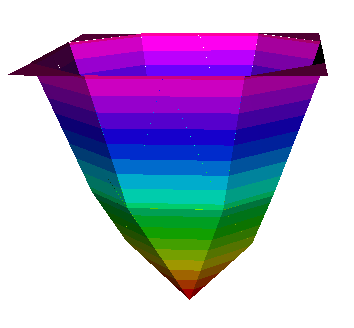
\includegraphics[scale=0.16]{img/Difusion/Recortes/steady_diffusion_exact_n_4.png}
				\caption{\scriptsize Exact.}
			\end{subfigure}
			\begin{subfigure}[b]{0.2\textwidth}
				\centering
				
\includegraphics[scale=0.16]{img/Difusion/Recortes/steady_diffusion_approx_n_4.png}
				\caption{\scriptsize Approx.}
			\end{subfigure}
			\begin{subfigure}[b]{0.1\textwidth}
				\centering
				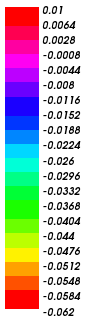
\includegraphics[scale=0.23]{img/Difusion/Recortes/steady_diffusion_values.png}
				%\caption*{ }
			\end{subfigure}
			\begin{subfigure}[b]{0.2\textwidth}
				\centering
				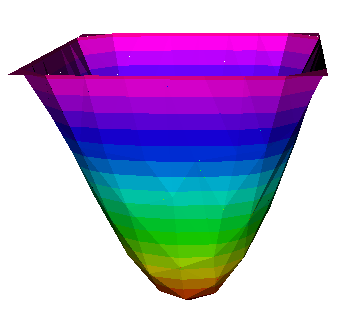
\includegraphics[scale=0.16]{img/Difusion/Recortes/steady_diffusion_exact_n_8.png}
				\caption{\scriptsize Exact.}
			\end{subfigure}
			\begin{subfigure}[b]{0.2\textwidth}
				\centering
				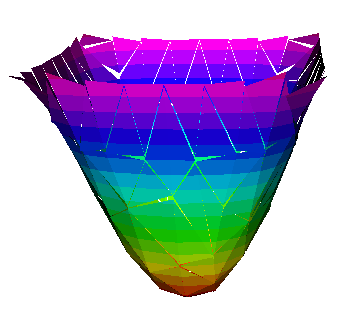
\includegraphics[scale=0.16]{img/Difusion/Recortes/steady_diffusion_approx_n_8.png}
				\caption{\scriptsize Approx.}
			\end{subfigure}
			\caption{\scriptsize Left, $h\approx\frac{1}{4}$. Right, $h\approx\frac{1}{8}$.}
		\end{figure}

		\begin{figure}[h!]
			\begin{subfigure}[b]{0.2\textwidth}
				\centering
				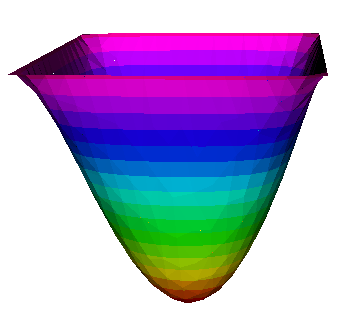
\includegraphics[scale=0.16]{img/Difusion/Recortes/steady_diffusion_exact_n_16.png}
				\caption{\scriptsize Exact.}
			\end{subfigure}
			\begin{subfigure}[b]{0.2\textwidth}
				\centering
				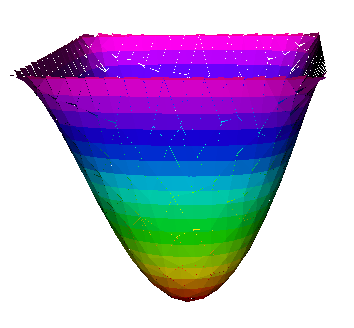
\includegraphics[scale=0.16]{img/Difusion/Recortes/steady_diffusion_approx_n_16.png}
				\caption{\scriptsize Approx.}
			\end{subfigure}
			\begin{subfigure}[b]{0.1\textwidth}
				\centering
				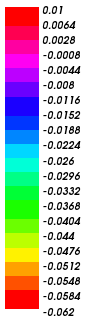
\includegraphics[scale=0.23]{img/Difusion/Recortes/steady_diffusion_values.png}
				%\caption*{ }
			\end{subfigure}
			\begin{subfigure}[b]{0.2\textwidth}
				\centering
				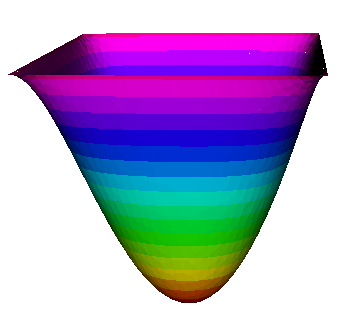
\includegraphics[scale=0.16]{img/Difusion/Recortes/steady_diffusion_exact_n_32.png}
				\caption{\scriptsize Exact.}
			\end{subfigure}
			\begin{subfigure}[b]{0.2\textwidth}
				\centering
				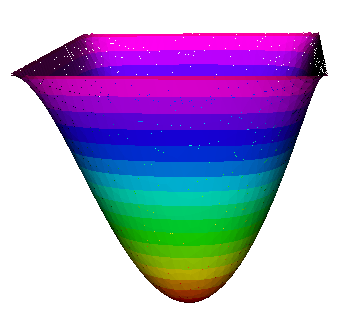
\includegraphics[scale=0.16]{img/Difusion/Recortes/steady_diffusion_approx_n_32.png}
				\caption{\scriptsize Approx.}
			\end{subfigure}
			\caption{\scriptsize Left, $h\approx\frac{1}{16}$. Right, $h\approx\frac{1}{32}$.}
		\end{figure}
		\end{frame}
		
		\begin{frame}{Errors with $\sigma=4$ and $\mathbb{P}^2_1(\T_h)$}
		\begin{minipage}{0.50\textwidth}
			\centering
			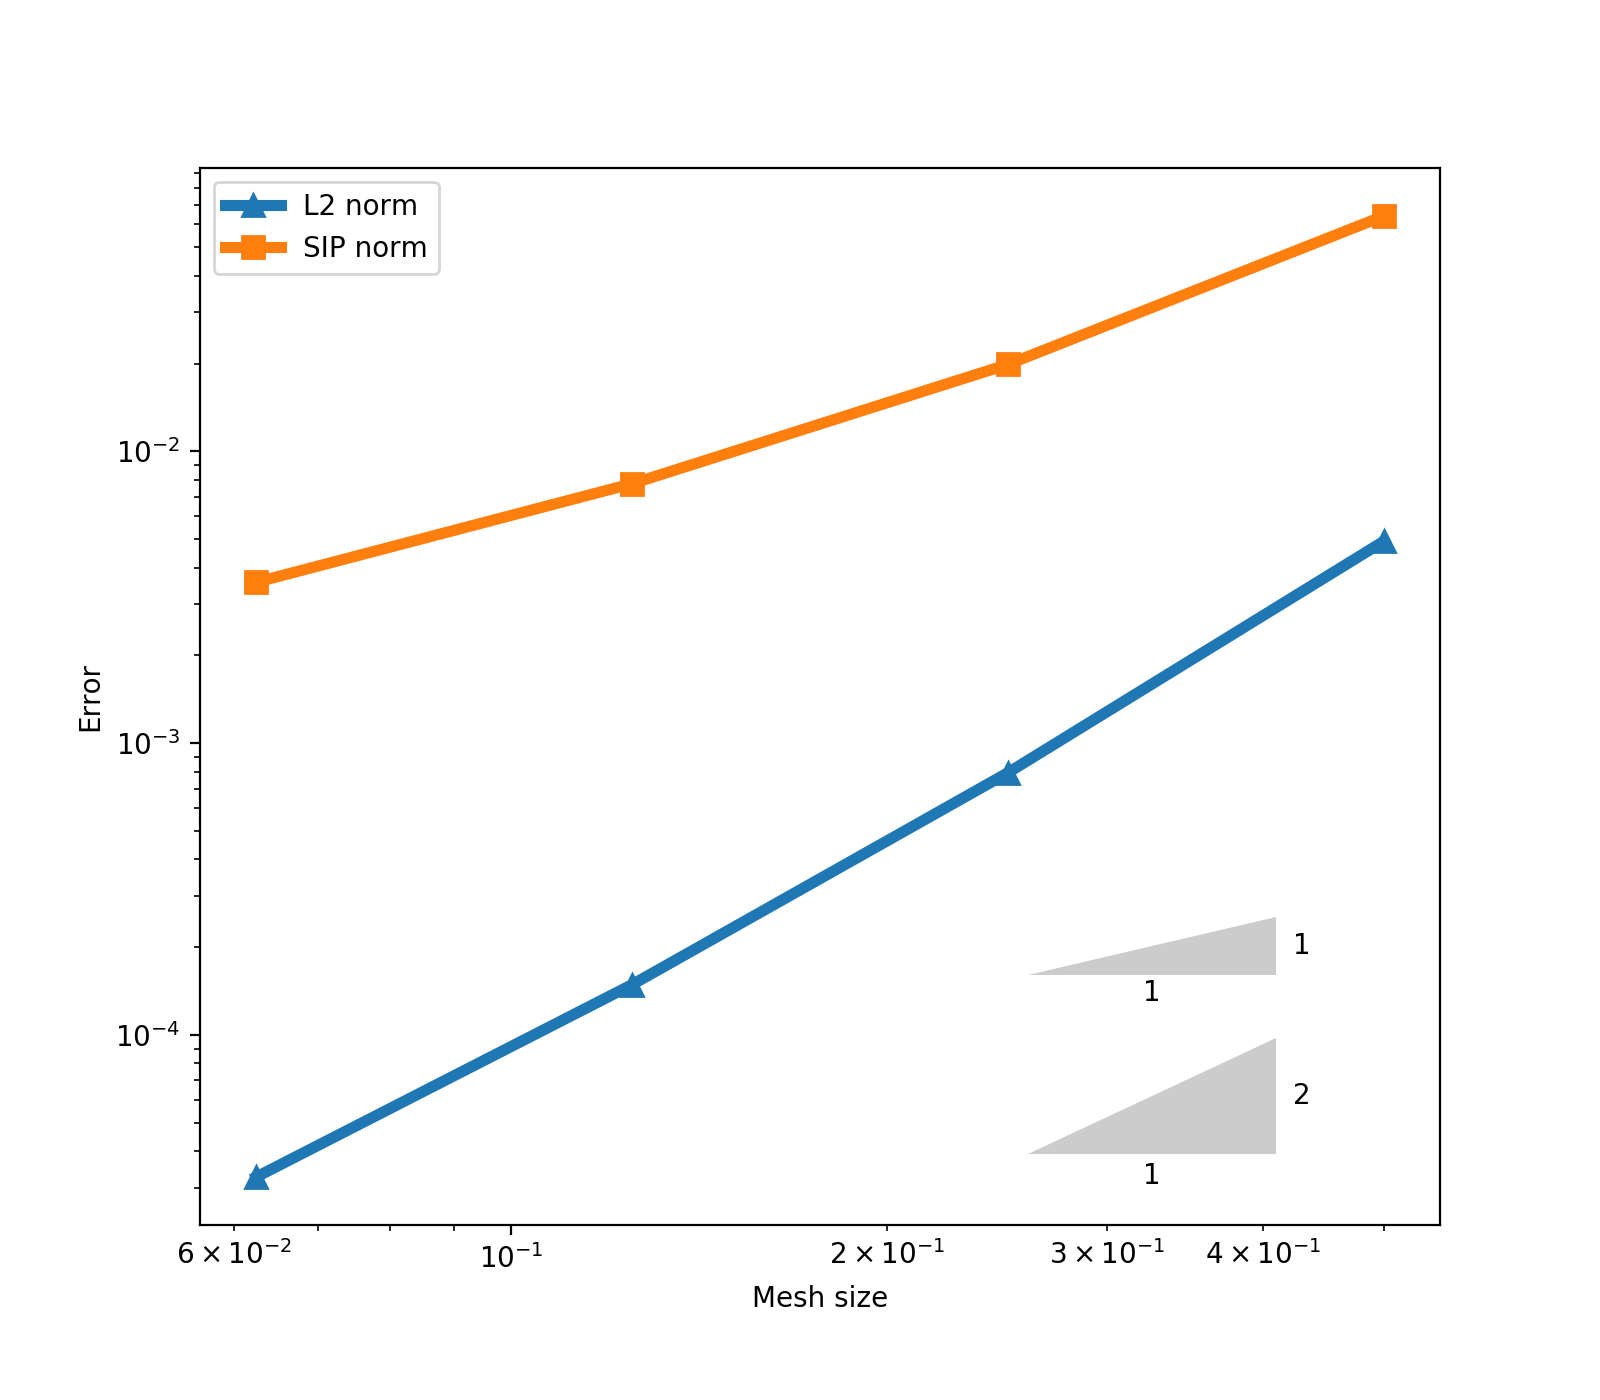
\includegraphics[scale=0.30]{img/Difusion/errores_difusion_P1dc.png}
			\captionof{figure}{Errors in logarithmic scale.}
		\end{minipage}
		\begin{minipage}{0.49\textwidth}
			\centering
			\begin{tabular}{|c|c|c|}
				\hline 
				\multirow{2}{*}{$h$} & \multicolumn{2}{c|}{Order} \\
				\cline{2-3}
				&  $\normasip{\cdot}$ & $\norma{\cdot}_{L^2(\Omega)}$ \\ 
				\hline
				\hline
				$\frac{1}{4}\to\frac{1}{8}$ & $1.69$ & $2.6$ \\ 
				\hline 
				$\frac{1}{8}\to\frac{1}{16}$ & $1.36$ & $2.41$ \\ 
				\hline 
				$\frac{1}{16}\to\frac{1}{32}$ & $1.12$ & $2.19$\\
				\hline
			\end{tabular}
			\captionof{table}{Convergence order.}
		\end{minipage}
		\end{frame}
		
		
		\begin{frame}{Errors with $\sigma=10$ and $\mathbb{P}^2_2(\T_h)$}
		\begin{minipage}{0.49\textwidth}
			\centering
			\begin{tabular}{|c|c|c|}
				\hline 
				\multirow{2}{*}{$h$} & \multicolumn{2}{c|}{Order} \\
				\cline{2-3}
				&  $\normasip{\cdot}$ & $\norma{\cdot}_{L^2(\Omega)}$ \\ 
				\hline
				\hline
				$\frac{1}{4}\to\frac{1}{8}$ & $2.24$ & $3.16$ \\ 
				\hline 
				$\frac{1}{8}\to\frac{1}{16}$ & $2.1$ & $3.06$ \\ 
				\hline 
				$\frac{1}{16}\to\frac{1}{32}$ & $1.95$ & $2.95$\\
				\hline
			\end{tabular}
			\captionof{table}{Order of convergence.}
		\end{minipage}
		\begin{minipage}{0.5\textwidth}
			\centering
			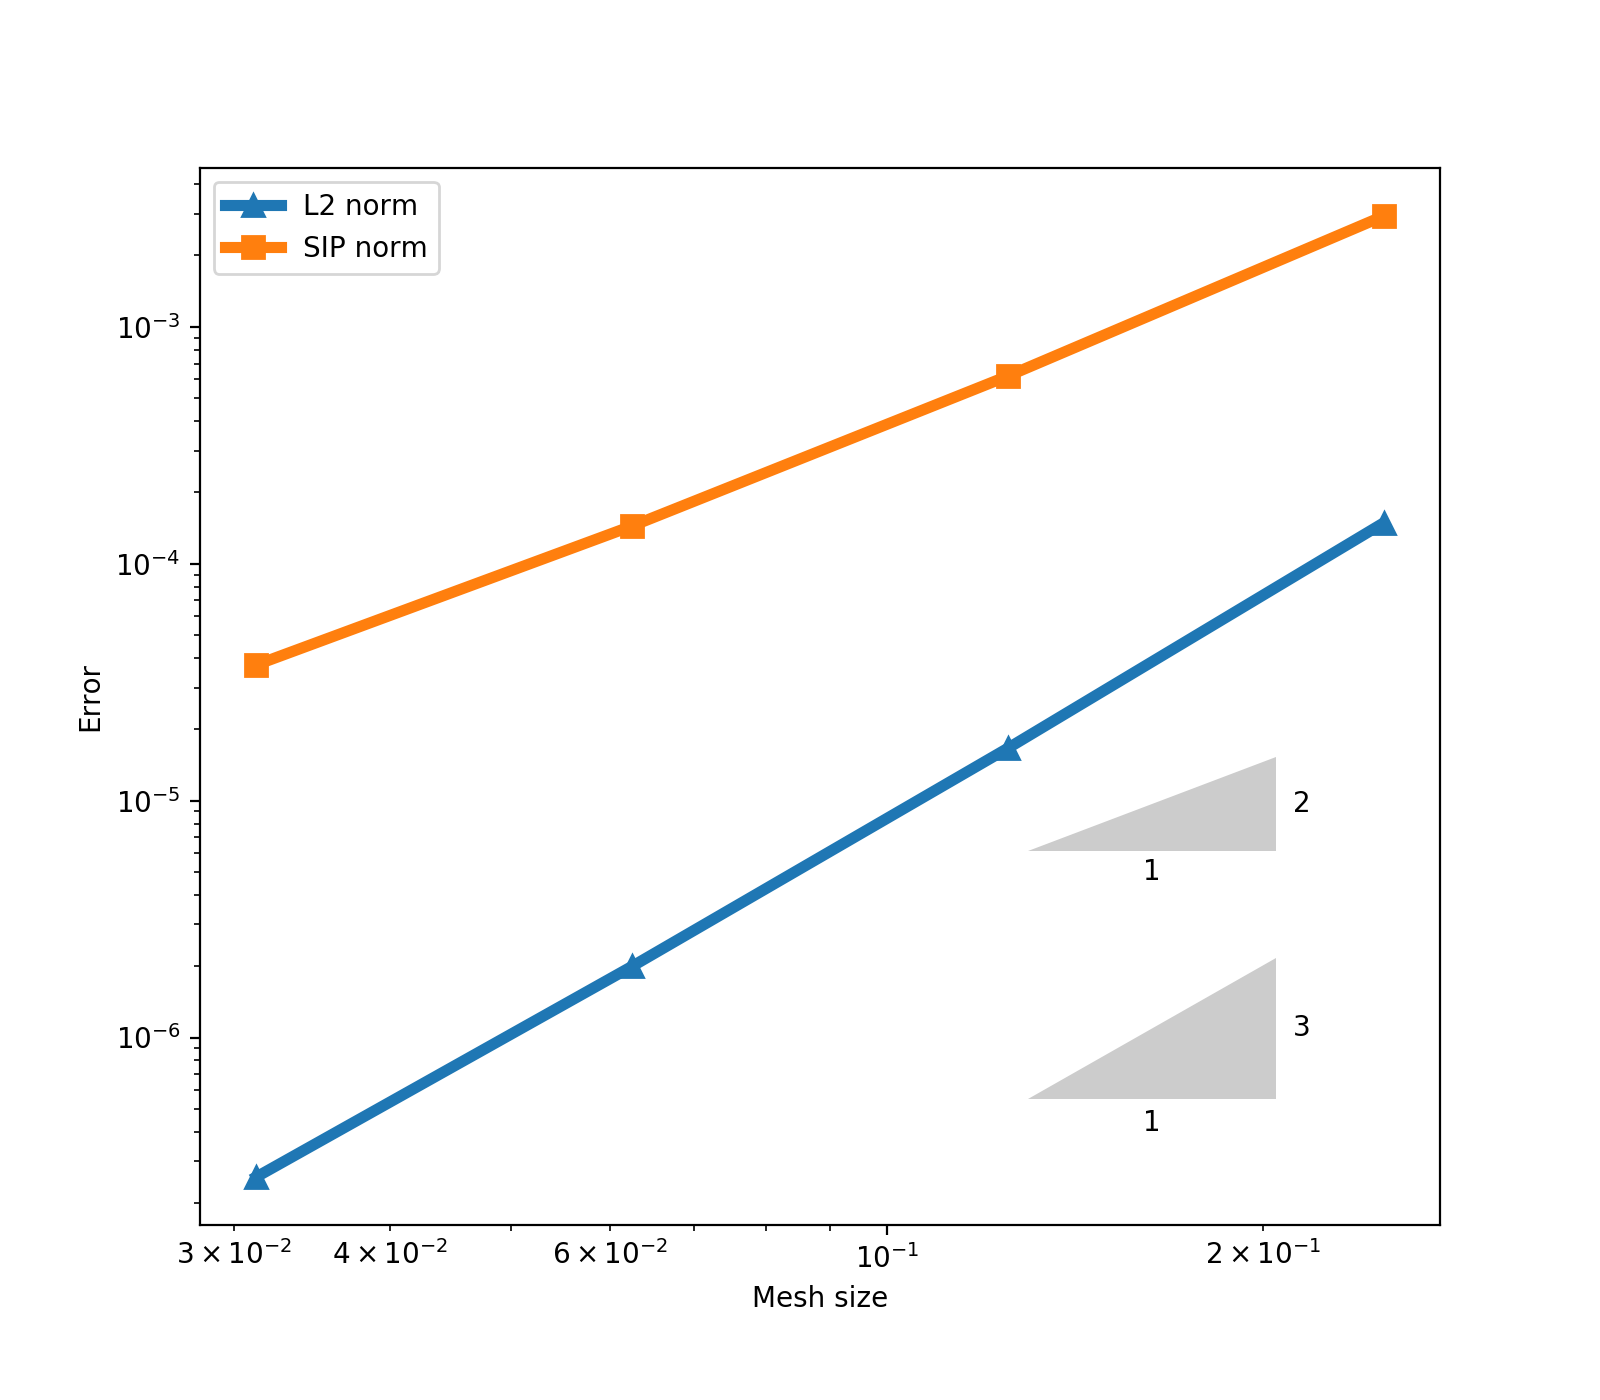
\includegraphics[scale=0.30]{img/Difusion/errores_difusion_P2dc.png}
			\captionof{figure}{Errors in logarithmic scale.}
		\end{minipage}
		\end{frame}
		
		\begin{frame}{Solutions with different $\sigma$ and $\mathbb{P}_1^2(\T_h)$}
		
		\begin{figure}[h!]
			\begin{subfigure}[b]{0.27\textwidth}
				\centering
				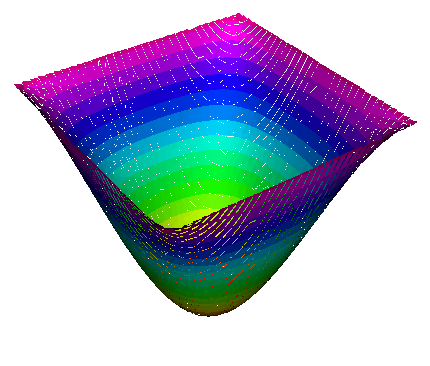
\includegraphics[scale=0.18]{img/Difusion/Recortes/steady_diffusion_approx_sigma_0_01.png}
				\caption{\scriptsize $\sigma=0,01$.}
			\end{subfigure}
			\begin{subfigure}[b]{0.27\textwidth}
				\centering
				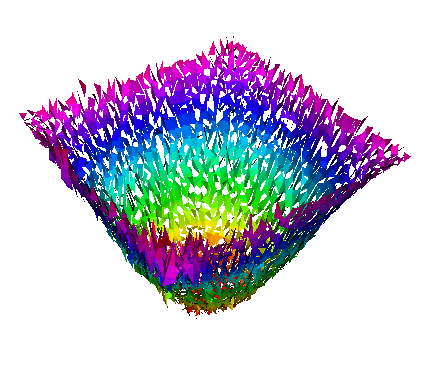
\includegraphics[scale=0.18]{img/Difusion/Recortes/steady_diffusion_approx_sigma_0_5.png}
				\caption{\scriptsize $\sigma=0,5$.}
			\end{subfigure}
			\begin{subfigure}[b]{0.27\textwidth}
				\centering
				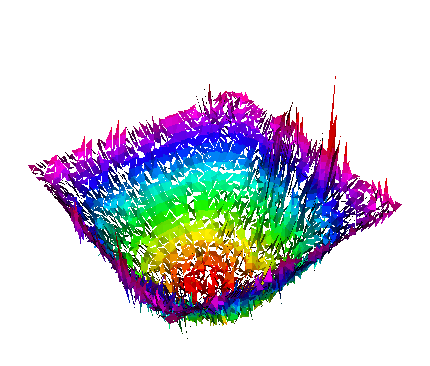
\includegraphics[scale=0.18]{img/Difusion/Recortes/steady_diffusion_approx_sigma_1.png}
				\caption{\scriptsize $\sigma=1$.}
			\end{subfigure}
			\begin{subfigure}[b]{0.15\textwidth}
				\centering
				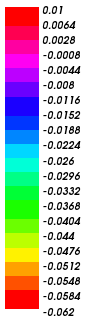
\includegraphics[scale=0.23]{img/Difusion/Recortes/steady_diffusion_values.png}
				%\caption*{ }
			\end{subfigure}
			%\end{figure}
			%\begin{figure}
			%	\ContinuedFloat
			\begin{subfigure}[b]{0.27\textwidth}
				\centering
				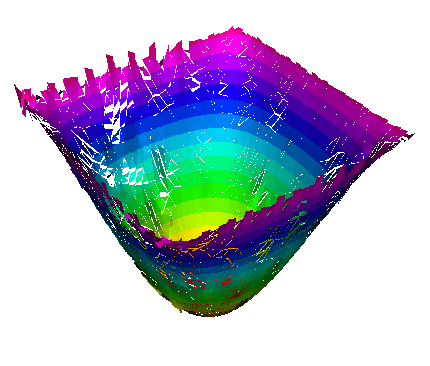
\includegraphics[scale=0.18]{img/Difusion/Recortes/steady_diffusion_approx_sigma_2.png}
				\caption{\scriptsize $\sigma=2$.}
			\end{subfigure}
			\begin{subfigure}[b]{0.27\textwidth}
				\centering
				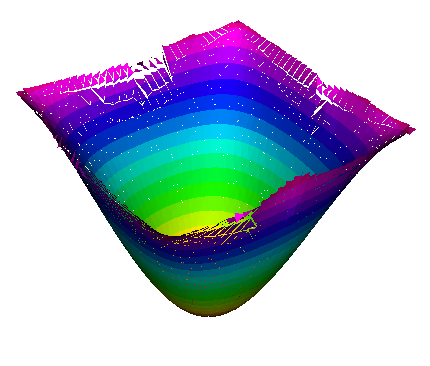
\includegraphics[scale=0.18]{img/Difusion/Recortes/steady_diffusion_approx_sigma_3.png}
				\caption{\scriptsize $\sigma=3$.}
			\end{subfigure}
			\begin{subfigure}[b]{0.27\textwidth}
				\centering
				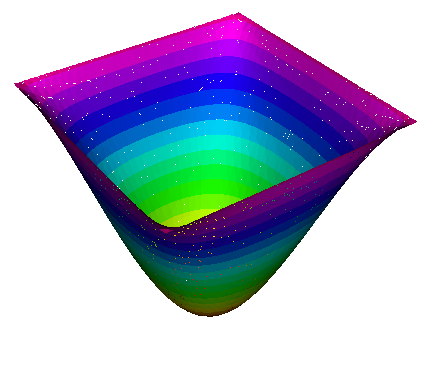
\includegraphics[scale=0.18]{img/Difusion/Recortes/steady_diffusion_approx_sigma_4.png}
				\caption{\scriptsize $\sigma=4$.}
			\end{subfigure}
			\begin{subfigure}[b]{0.15\textwidth}
				\centering
				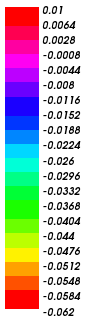
\includegraphics[scale=0.23]{img/Difusion/Recortes/steady_diffusion_values.png}
				%\caption*{ }
			\end{subfigure}
			\caption{\scriptsize Discrete solutions with $h\approx\frac{1}{32}$.}
		\end{figure}
		
		\end{frame}
		
		\begin{frame}{Errors with different $\sigma$ and $\mathbb{P}_1^2(\T_h)$}
			\begin{figure}[h!]
				\centering
				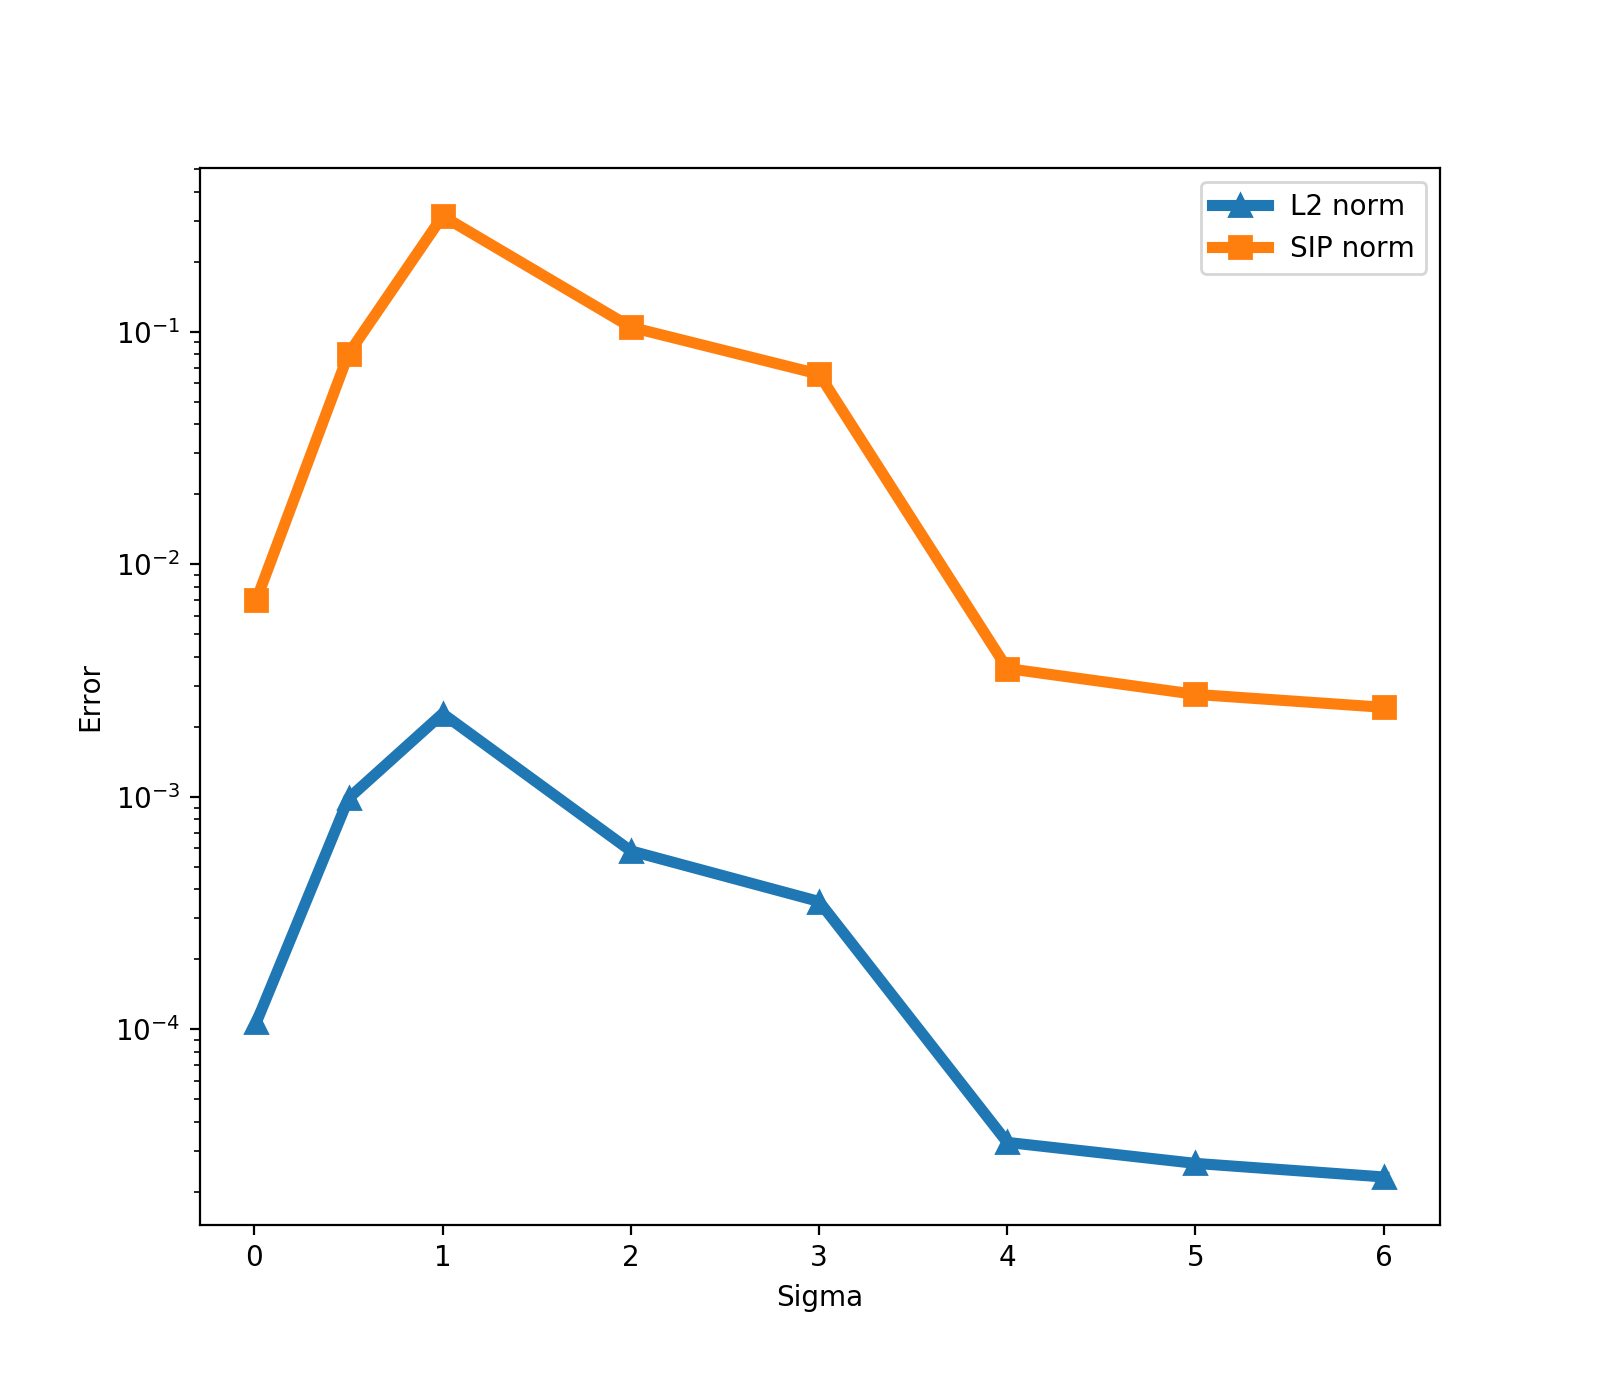
\includegraphics[scale=0.37]{img/Difusion/errores_difusion_sigma.png}
				\caption{Errors with $h\approx\frac{1}{32}$.}
			\end{figure}
		\end{frame}

	\subsection{Hyperbollic problem}
	
	\begin{frame}{Model problem}
		We consider the convection-reaction problem:
		\begin{block}{}
		\begin{equation*}
		\left\{
		\begin{aligned}
		\beta\cdot\nabla u+\mu u&=f & \text{in } &\Omega, \\
		u&=0 & \text{on } &\partial\Omega^-,
		\end{aligned}
		\right.
		\end{equation*}
		\end{block}
		where 
		\begin{itemize}
			\item $\partial\Omega^-=\left\{x\in\partial\Omega\colon \beta(x)\mathbf{n}(x)<0\right\},$
			\item $\mu\in L^\infty(\Omega)$,
			\item $\beta\in\left[\text{Lip}(\Omega)\right]^d \Rightarrow \norma{\nabla\beta_i}_{L^\infty(\Omega)^d}\le C_\beta$ for some $C_\beta >0$.
			\item $f\in L^2(\Omega)$.
		\end{itemize}
		\vspace*{.5cm}
		We assume that there is $\mu_0>0$ such that $\displaystyle\mu-\frac{1}{2}\nabla\cdot\beta\geq\mu_0$ in $\Omega$.
		
		\end{frame}

	\subsubsection{Numerical approximation}
	
	\begin{frame}{Finite-dimensional space}
	
	\textbf{Finite-dimensional space}: $$V_h\coloneqq\alert{\mathbb{P}_k^d(\T_h)}$$ with basis $\left\{\phi_i\right\}_{i=1}^{N_h^{\text{cf}}}$.
	\vspace*{1cm}
	
	We denote:
	\begin{itemize}
		\item $V_*\coloneqq V\cap H^1(\T_h)$;
		\item $V_{*h}\coloneqq V_*+V_h$.
	\end{itemize}
	\end{frame}
	
	\begin{frame}{Centered Fluxes Method}
	\begin{itemize}\itemsep1em
		\item $a_h^{\text{cf}}\colon V_{*h}\times V_h\to\R$,
		\begin{align*}
		\alert{\acf{u}{v_h}}&\coloneqq\framedmath<2>{\displaystyle \int_\Omega(\beta\cdot\nabla_h u)v_h+\int_\Omega\mu u v_h}\\&\framedmath<3>{\displaystyle +\int_{\partial\Omega}(\beta\cdot\mathbf{n})^\ominus uv_h}\framedmath<4>{\displaystyle -\sum_{e\in\E_h^i}\int_e(\beta\cdot\mathbf{n}_e)\salto{u}\media{v_h}},
		\end{align*}
		where $(w)^\ominus=\frac{\vert w\vert - w}{2}$.
		\vspace*{0.3cm}
		\begin{itemize}
			\item<2> \myframed{Terms of the model.}
			\item<3> \myframed{Weak boundary conditions.}
			\item<4> \myframed{Coercivity.}
		\end{itemize}
		\item $L_h\colon V_h\to\R$, $\displaystyle \alert{L_h(v_h)}\coloneqq\int_\Omega f v_h.$
	\end{itemize}
\end{frame}

\begin{frame}{Discrete problem}
	\begin{itemize}
		\item $\text{Find }u_h\in V_h\text{ such that }\acf{u_h}{v_h}=L_h(v_h)\text{ for every }v_h\in V_h$.
	\end{itemize}
	\vspace*{0.1cm}
	$$\Big{\Updownarrow}$$
	\vspace*{-0.3cm}
	\begin{itemize}
		\item Solve the linear system $A^{\text{cf}}\mathbf{U}^{\text{cf}}=\mathbf{F}^{\text{cf}}$ where:
		\vspace*{0.3cm}
		\begin{itemize}
			\item $A^{\text{cf}}=\left(A_{ij}^{\text{cf}}\right)_{i,j\in\left\{1,2,\ldots,N_h^{\text{cf}}\right\}}$ with $A_{ij}^{\text{cf}}=\acf{\phi_j}{\phi_i}$;
			\item $\mathbf{U}^{\text{cf}}=\left(U_1^{\text{cf}},U_2^{\text{cf}},\ldots,U_{N_h^{\text{cf}}}^{\text{cf}}\right)^t$ with $u_h=\displaystyle\sum_{i=1}^{N_h^{\text{cf}}}U_i^{\text{cf}}\phi_i$;
			\item $\mathbf{F}^{\text{cf}}=\left(F_1^{\text{cf}},F_2^{\text{cf}},\ldots,F_{N_h^{\text{cf}}}^{\text{cf}}\right)^t$ with $F_i^{\text{cf}}=L_h(\phi_i)$.
		\end{itemize}
	\end{itemize}
	
	\vspace*{0.3cm}
	The model problem and the discrete problem are \alert{equivalent} in $H^1(\Omega)$.
	
	\end{frame}
	
	\begin{frame}[allowframebreaks]{Properties of the discrete problem}
	\begin{definicion}
		In the space $V_{*h}$ we define the norm $\normacf{\cdot}\colon V_{*h}\to\R$ as {\small $$\normacf{u}\coloneqq\escalarcf{u}{u}^{1/2}= \left(\max\{\norma{\mu}_{L^\infty(\Omega)},C_\beta\}\norma{u}_{L^2(\Omega)}^2+\frac{1}{2}\norma{u}_{L^2(|\beta\cdot\mathbf{n}|;\partial\Omega)}^2\right)^{1/2}.$$}
	\end{definicion}
	\framebreak
	\begin{lemma}
		The bilinear form $\acf{\cdot}{\cdot}$ is continuous in $V_h$ with the norm $\normacf{\cdot}$, i.e., there is $C>0$ such that for every $u_h,v_h\in V_h$ it holds that $$\acf{u_h}{v_h}\leq C\normacf{u_h}\normacf{v_h}.$$
	\end{lemma}
	
	\begin{lemma}
		The bilinear form $\acf{\cdot}{\cdot}$ is coercitive in $V_h$ with the norm $\normacf{\cdot}$, i.e., there is $C>0$ such that for every $v_h\in V_h$ it holds that $$\acf{v_h}{v_h}\geq C\normacf{v_h}^2.$$
	\end{lemma}
	\framebreak
	\begin{lemma}
		There is a unique solution $u_h\in V_h$ of the discrete problem $$\acf{u_h}{v_h}=L_h(v_h)$$ for every $v_h\in V_h$.
	\end{lemma}
	% \textbf{Demostraciones}:
	% \begin{enumerate}
	% 	\item Lax-Milgram.
	% 	\item Unicidad de solución.
	% \end{enumerate}
	
	\end{frame}
	
	\begin{frame}{Error analysis}
	\begin{theorem}
		\label{theorem:hiperbolico_CF_orden_norma_CF}
		Let $u\in H^{k+1}(\Omega)$, $k\in\N$ be the solution of the model problem and $u_h\in \mathbb{P}_k^d(\T_h)$ the solution of the discrete problem.
		
		Then, there is $C>0$ independent of $h$ and depending on the data only through the factor $\left(\min\{1,\max\{\norma{\mu}_{L^\infty(\Omega)},C_\beta\}\mu_0\}\right)^{-1}$ so that
		\begin{equation*}
		\label{theorem:orden_convergencia_CF}
		\normacf{u-u_h}\leq C\norma{u}_{H^{k+1}(\Omega)}h^k.
		\end{equation*}
	\end{theorem}
	\end{frame}
	
	\begin{frame}{Upwind Method}
	
	\begin{itemize}\itemsep1em
		\item $a_h^{\text{upw}}\colon V_{*h}\times V_h\to \R$, $$\alert{\aupw{u}{v_h}}\coloneqq \framedmath<2>{\displaystyle \acf{u}{v_h}}+\framedmath<3>{\displaystyle \sum_{e\in\E_h^i}\int_e\frac{\eta}{2}|\beta\cdot\mathbf{n}_e|\salto{u}\salto{v_h}};$$
		\begin{itemize}
			\item<2> \myframed{Centered Fluxes Method.}
			\item<3> \myframed{Stability.}
		\end{itemize}
		\item $L_h\colon V_h\to\R$, $\displaystyle \alert{L_h(v_h)}\coloneqq\int_\Omega f v_h.$
	\end{itemize}
	\end{frame}
	
	\begin{frame}{Problema discreto}
	
	\begin{itemize}
		\item $\text{Find }u_h\in V_h\text{ such that }\aupw{u_h}{v_h}=L_h(v_h)\text{ for every }v_h\in V_h$.
	\end{itemize}
	\vspace*{0.1cm}
	$$\Big{\Updownarrow}$$
	\vspace*{-0.3cm}
	\begin{itemize}
		\item Solve the linear system $A^{\text{upw}}\mathbf{U}^{\text{upw}}=\mathbf{F}^{\text{upw}}$ where:
		\vspace*{0.3cm}
		\begin{itemize}
			\item $A^{\text{upw}}=\left(A_{ij}^{\text{upw}}\right)_{i,j\in\left\{1,2,\ldots,N_h^{\text{upw}}\right\}}$ with $A_{ij}^{\text{upw}}=\aupw{\phi_j}{\phi_i}$;
			\item $\mathbf{U}^{\text{upw}}=\left(U_1^{\text{upw}},U_2^{\text{upw}},\ldots,U_{N_h^{\text{upw}}}^{\text{upw}}\right)^t$ with $u_h=\displaystyle\sum_{i=1}^{N_h^{\text{upw}}}U_i^{\text{upw}}\phi_i$;
			\item $\mathbf{F}^{\text{upw}}=\left(F_1^{\text{upw}},F_2^{\text{upw}},\ldots,F_{N_h^{\text{upw}}}^{\text{upw}}\right)^t$ with $F_i^{\text{upw}}=L_h(\phi_i)$.
		\end{itemize}
	\end{itemize}
	
	\vspace*{0.3cm}
	The model problem and the discrete problem are \alert{equivalent} in $H^1(\Omega)$.
	
	\end{frame}
	
	\begin{frame}[allowframebreaks]{Properties of the discrete problem}
	\begin{definicion}
		In the space $V_{*h}$ we define the norm $\normaupw{\cdot}\colon V_{*h}\to\R$ as $$\normaupw{u}\coloneqq\escalarupw{u}{u}^{1/2}= \left(\normacf{u}^2+\frac{\eta}{2}\sum_{e\in\E_h^i}\norma{\salto{u}}^2_{L^2(|\beta\cdot\mathbf{n}_e|;e)} \right)^{1/2}.$$
	\end{definicion}
	\framebreak
	\begin{lemma}
		The bilinear form $\aupw{\cdot}{\cdot}$ is continuous in $V_h$ with the norm $\normaupw{\cdot}$, i.e., there is $C>0$ such that for every $u_h,v_h\in V_h$ it holds that $$\aupw{u_h}{v_h}\leq C\normaupw{u_h}\normaupw{v_h}.$$
	\end{lemma}
	
	\begin{proposition}
		The bilinear form $\aupw{\cdot}{\cdot}$ is coercive in $V_h$ with the norm $\normaupw{\cdot}$, i.e., there is $C>0$ such that for every $v_h\in V_h$ it holds that $$\aupw{v_h}{v_h}\geq C\normaupw{v_h}^2.$$
	\end{proposition}
	\framebreak
	\begin{lemma}
		There is a unique solution $u_h\in V_h$ of the discrete problem $$\aupw{u_h}{v_h}=L_h(v_h)$$ for every $v_h\in V_h$.
	\end{lemma}
	% \textbf{Demostraciones}:
	% \begin{enumerate}
	% 	\item Lax-Milgram.
	% 	\item Unicidad de solución.
	% \end{enumerate}
	\end{frame}
	
	\begin{frame}{Error analysis}
	\begin{theorem}
		Let $u\in H^{k+1}(\Omega)$, $k\in\N$ the solution of the model problem and $u_h\in \mathbb{P}_k^d(\T_h)$ the solution of the discrete problem.
		
		Then, there is $C>0$ independent of $h$ and depending on the data only through the factor  $\left(\min\{1,\max\{\norma{\mu}_{L^\infty(\Omega)},C_\beta\}\mu_0\}\right)^{-1}$ such that $$\normaupw{u-u_h}\leq C\norma{u}_{H^{k+1}(\Omega)}h^{k+1/2}.$$
	\end{theorem}
\end{frame}

	\subsubsection{Numerical experiments}
	\begin{frame}{Hyperbolic problem}
		\scriptsize
		We consider the hyperbolic problem:
		\begin{block}{}
		\begin{equation*}
		\left\{
		\begin{aligned}
		\beta\cdot\nabla u+\mu u&=f & \text{en } &\Omega, \\
		u&=0 & \text{en } &\partial\Omega^-,
		\end{aligned}
		\right.
		\end{equation*}
		\end{block}
		with
		\begin{itemize}
			\item $d=2$;
			\item $\Omega=\left\{(x,y)\in\R^2\colon x^2+y^2<1 \right\}$;
			\item $A=10$, $x_0=y_0=0.3$;
			\item $\mu=2A$;
			\item $\beta(x,y)\coloneqq(y,-x)$;
			\item $f\colon\Omega\to\R$, $f(x,y)\coloneqq \mu e^{-A\left((x-x_0)^2+(y-y_0)^2\right)}(x_0 y -x y_0 + 1)$.
		\end{itemize}
		
		\vspace*{0.3cm}
		$u_{\text{ex}}\colon\Omega\to\R$ defined as
		\begin{equation*}
		\label{sol_experimento_hiperbolico}
		\uex (x,y)\coloneqq e^{-A\left((x-x_0)^2+(y-y_0)^2\right)}
		\end{equation*}
		is the \alert{unique exact solution} ($\alert{u_\text{ex}\in V}$).
		
		\end{frame}
		
		\begin{frame}{Solutions with $\mathbb{P}_1^2(\T_h)$}
		\vspace{-0.2cm}
		\begin{figure}[h!]
			\begin{subfigure}[b]{0.27\textwidth}
				\centering
				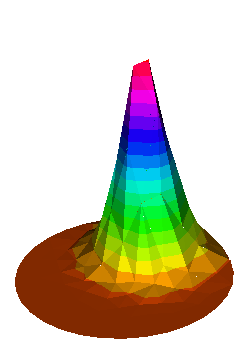
\includegraphics[scale=0.2]{img/Conveccion_Reaccion/Recortes/steady_convect_react_exact_n_32.png}
				\caption{Exact.}
			\end{subfigure}
			\begin{subfigure}[b]{0.27\textwidth}
				\centering
				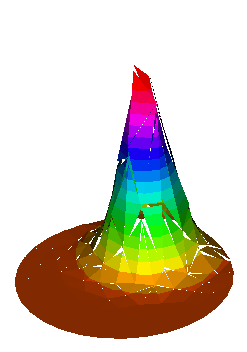
\includegraphics[scale=0.2]{img/Conveccion_Reaccion/Recortes/steady_convect_react_approx_CF_n_32.png}
				\caption{Centered fluxes.}
			\end{subfigure}
			\begin{subfigure}[b]{0.27\textwidth}
				\centering
				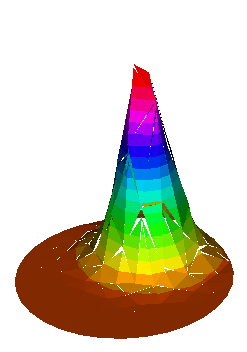
\includegraphics[scale=0.2]{img/Conveccion_Reaccion/Recortes/steady_convect_react_approx_UPW_n_32.png}
				\caption{Upwind.}
			\end{subfigure}
			\begin{subfigure}[b]{0.15\textwidth}
				\centering
				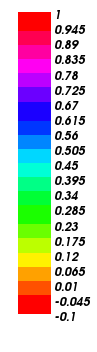
\includegraphics[scale=0.2]{img/Conveccion_Reaccion/Recortes/steady_convect_react_values.png}
				%\caption*{ }
			\end{subfigure}
			\caption{Solutions obtained with $h\approx\frac{\pi}{16}$.}
		\end{figure}
		\vspace{-0.7cm}
		\begin{figure}[h!]
			\begin{subfigure}[b]{0.27\textwidth}
				\centering
				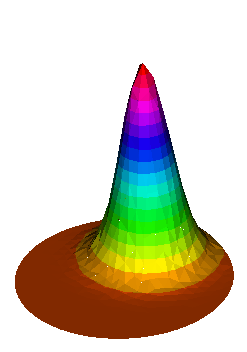
\includegraphics[scale=0.2]{img/Conveccion_Reaccion/Recortes/steady_convect_react_exact_n_64.png}
				\caption{Exact.}
			\end{subfigure}
			\begin{subfigure}[b]{0.27\textwidth}
				\centering
				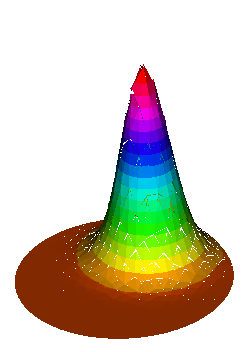
\includegraphics[scale=0.2]{img/Conveccion_Reaccion/Recortes/steady_convect_react_approx_CF_n_64.png}
				\caption{Centered fluxes.}
			\end{subfigure}
			\begin{subfigure}[b]{0.27\textwidth}
				\centering
				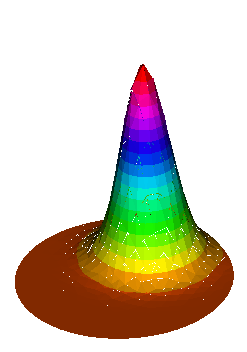
\includegraphics[scale=0.2]{img/Conveccion_Reaccion/Recortes/steady_convect_react_approx_UPW_n_64.png}
				\caption{Upwind.}
			\end{subfigure}
			\begin{subfigure}[b]{0.15\textwidth}
				\centering
				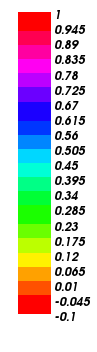
\includegraphics[scale=0.2]{img/Conveccion_Reaccion/Recortes/steady_convect_react_values.png}
				%\caption*{ }
			\end{subfigure}
			\caption{Solutions obtained with $h\approx\frac{\pi}{32}$.}
		\end{figure}
		\end{frame}
		
		\begin{frame}{Solutions with $\mathbb{P}_1^2(\T_h)$}
		\vspace{-0.2cm}
		\begin{figure}[h!]
			\begin{subfigure}[b]{0.27\textwidth}
				\centering
				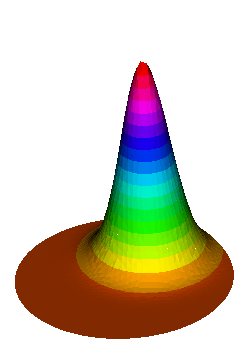
\includegraphics[scale=0.22]{img/Conveccion_Reaccion/Recortes/steady_convect_react_exact_n_128.png}
				\caption{Exact.}
			\end{subfigure}
			\begin{subfigure}[b]{0.27\textwidth}
				\centering
				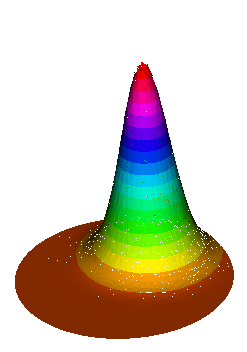
\includegraphics[scale=0.22]{img/Conveccion_Reaccion/Recortes/steady_convect_react_approx_CF_n_128.png}
				\caption{Centered fluxes.}
			\end{subfigure}
			\begin{subfigure}[b]{0.27\textwidth}
				\centering
				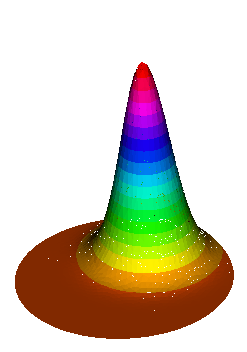
\includegraphics[scale=0.22]{img/Conveccion_Reaccion/Recortes/steady_convect_react_approx_UPW_n_128.png}
				\caption{Upwind.}
			\end{subfigure}
			\begin{subfigure}[b]{0.15\textwidth}
				\centering
				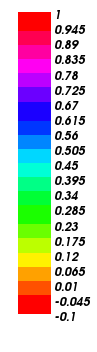
\includegraphics[scale=0.22]{img/Conveccion_Reaccion/Recortes/steady_convect_react_values.png}
				%\caption*{ }
			\end{subfigure}
			\caption{Solutions obtained with $h\approx\frac{\pi}{64}$.}
		\end{figure}
		\vspace{-0.7cm}
		\begin{figure}[h!]
			\begin{subfigure}[b]{0.27\textwidth}
				\centering
				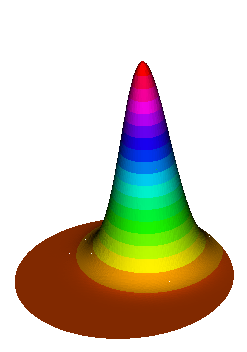
\includegraphics[scale=0.22]{img/Conveccion_Reaccion/Recortes/steady_convect_react_exact_n_256.png}
				\caption{Exact.}
			\end{subfigure}
			\begin{subfigure}[b]{0.27\textwidth}
				\centering
				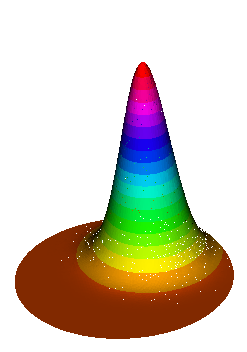
\includegraphics[scale=0.22]{img/Conveccion_Reaccion/Recortes/steady_convect_react_approx_CF_n_256.png}
				\caption{Centered fluxes.}
			\end{subfigure}
			\begin{subfigure}[b]{0.27\textwidth}
				\centering
				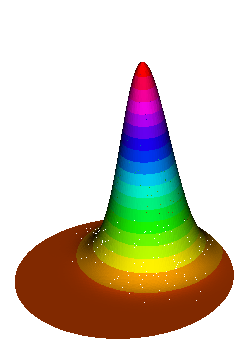
\includegraphics[scale=0.22]{img/Conveccion_Reaccion/Recortes/steady_convect_react_approx_UPW_n_256.png}
				\caption{Upwind.}
			\end{subfigure}
			\begin{subfigure}[b]{0.15\textwidth}
				\centering
				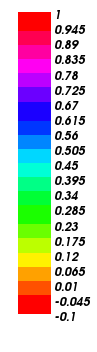
\includegraphics[scale=0.22]{img/Conveccion_Reaccion/Recortes/steady_convect_react_values.png}
				%\caption*{ }
			\end{subfigure}
			\caption{Solutions obtained with $h\approx\frac{\pi}{128}$.}
		\end{figure}
		\end{frame}
		
		\begin{frame}{Errors with $\mathbb{P}_1^2(\T_h)$}
		\hspace{-0.3cm}
		\begin{minipage}{0.5\textwidth}
			\centering
			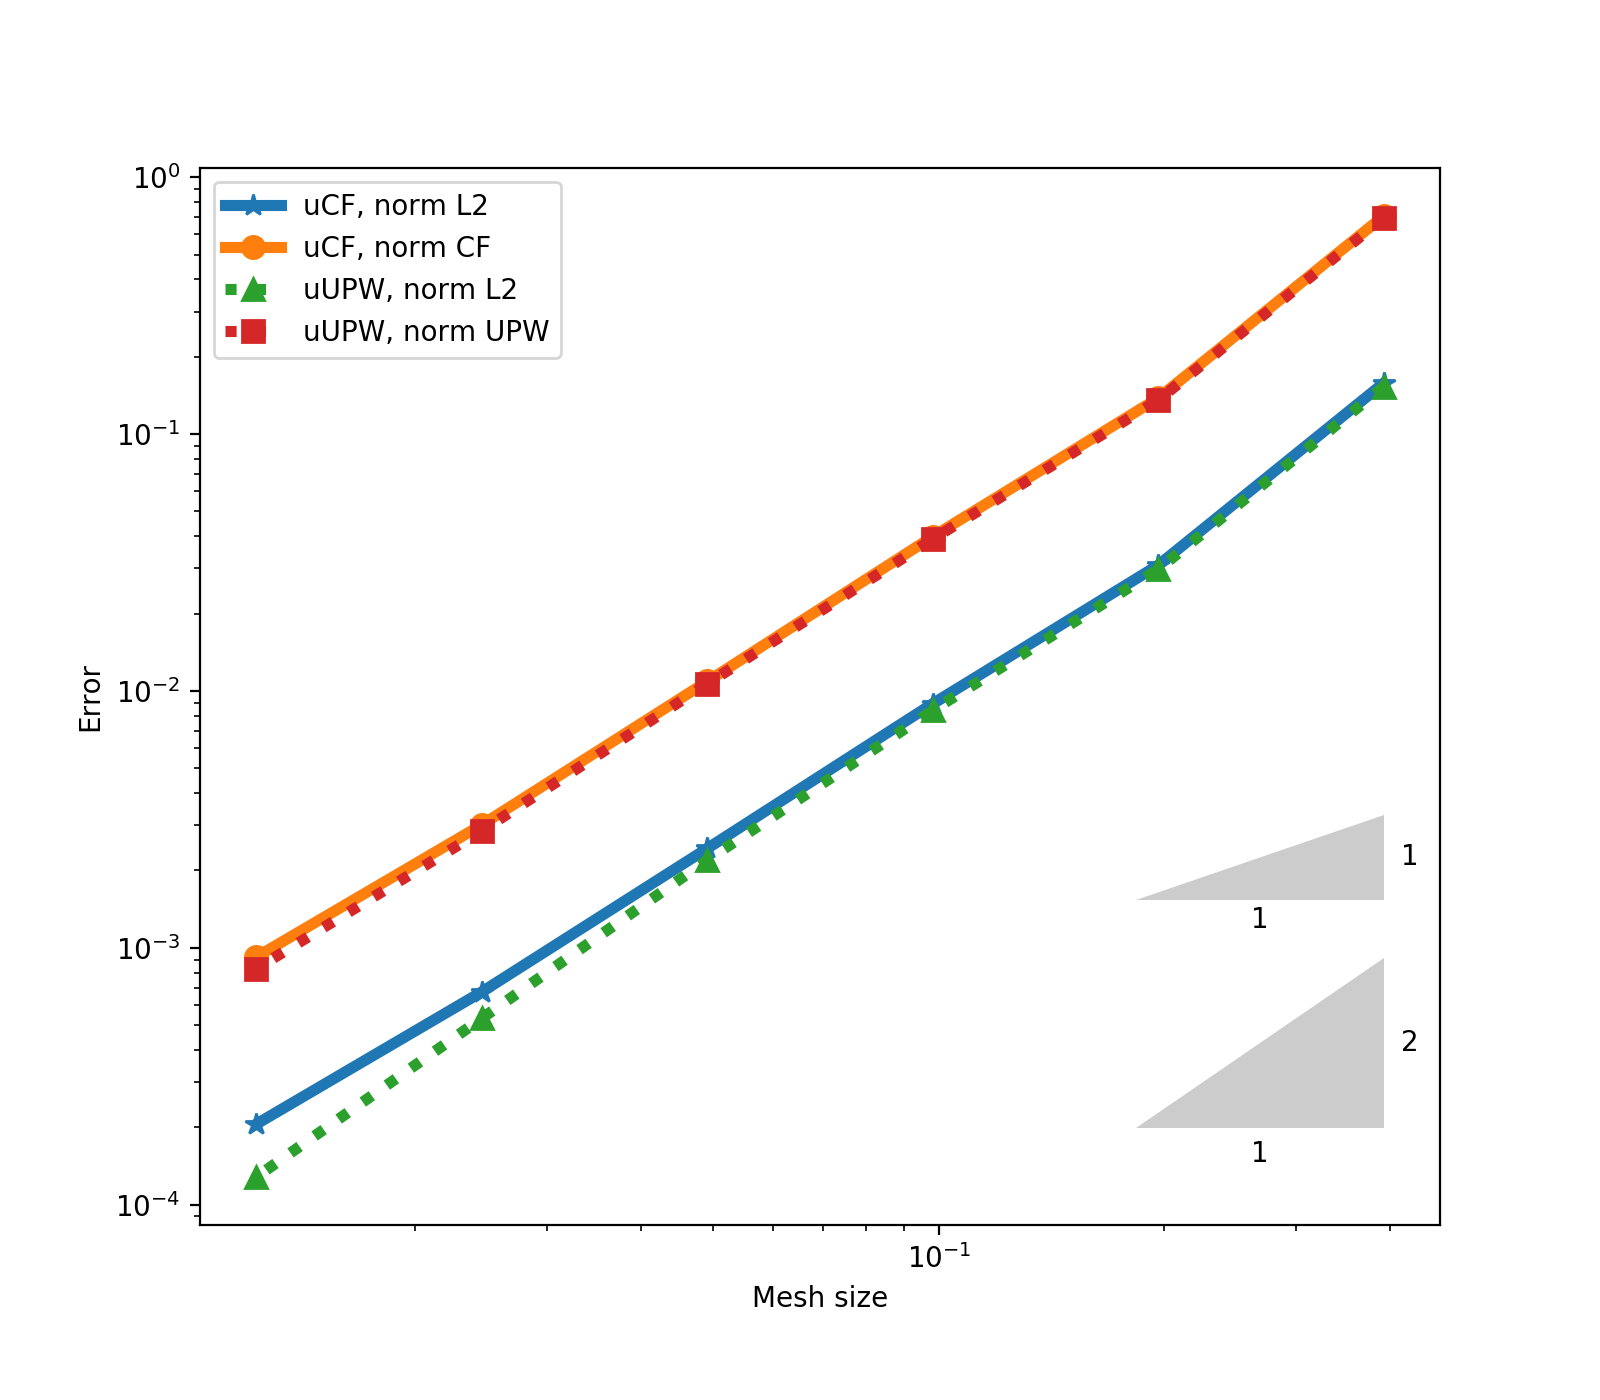
\includegraphics[scale=0.30]{img/Conveccion_Reaccion/errores_conveccion_reaccion_P1dc.png}
			\captionof{figure}{Errors in logarithmic scale.}
		\end{minipage}
		\begin{minipage}{0.49\textwidth}
			\scriptsize
			\centering
				\begin{tabular}{|c|c|c|c|}
					\hline
					\multirow{2}{*}{$h$} & \multicolumn{2}{c|}{Order} & \multirow{2}{*}{Method}\\
					\cline{2-3}
					& $\norma{\cdot}_*$ & $\norma{\cdot}_{L^2(\Omega)}$ & \\ 
					\hline
					\hline
					\multirow{2}{*}{$\frac{\pi}{8}\to\frac{\pi}{16}$} & $2.36$ & $2.36$ & CF\\
					\cdashline{2-4}
					& $2.36$ & $2.36$ & UPW\\ 
					\hline 
					\multirow{2}{*}{$\frac{\pi}{16}\to\frac{\pi}{32}$} & $1.79$ & $1.79$ & CF\\
					\cdashline{2-4}
					
					& $1.79$ & $1.82$ & UPW\\
					\hline 
					\multirow{2}{*}{$\frac{\pi}{32}\to\frac{\pi}{64}$} & $1.87$ & $1.87$ & CF\\
					\cdashline{2-4}
					
					& $1.87$ & $1.94$ & UPW\\
					\hline
					\multirow{2}{*}{$\frac{\pi}{64}\to\frac{\pi}{128}$} & $1.85$ & $1.85$ & CF\\
					\cdashline{2-4}
					
					& $1.9$ & $2.04$ & UPW\\
					\hline
					\multirow{2}{*}{$\frac{\pi}{128}\to\frac{\pi}{256}$} & $1.71$ & $1.71$ & CF\\
					\cdashline{2-4}
					
					& $1.78$ & $2.05$& UPW\\
					\hline
				\end{tabular}
			%\captionof{table}{Orden de convergencia en cada iteración para ambos métodos en normas $\normacf{\cdot}$ o $\normaupw{\cdot}$ y $\norma{\cdot}_{L^2(\Omega)}$ con espacio discreto $\mathbb{P}^2_1(\T_h)$.}
			\captionof{table}{Order of convergence.}
		\end{minipage}
		
		\end{frame}
		
		\begin{frame}{Errors with $\mathbb{P}_2^2(\T_h)$}
		\hspace*{-0.5cm}
		\begin{minipage}{0.48\textwidth}
			\scriptsize
			\centering
				\begin{tabular}{|c|c|c|c|}
					\hline
					\multirow{2}{*}{$h$} & \multicolumn{2}{c|}{Orden} & \multirow{2}{*}{Method}\\
					\cline{2-3}
					& $\norma{\cdot}_*$ & $\norma{\cdot}_{L^2(\Omega)}$ & \\ 
					\hline
					\hline
					\multirow{2}{*}{$\frac{\pi}{8}\to\frac{\pi}{16}$} & $2.72$ & $2.72$ & CF\\
					\cdashline{2-4}
					& $2.69$ & $2.73$ & UPW\\ 
					\hline 
					\multirow{2}{*}{$\frac{\pi}{16}\to\frac{\pi}{32}$} & $2.8$ & $2.8$ & CF\\
					\cdashline{2-4}
					
					& $2.73$ & $2.84$ & UPW\\
					\hline 
					\multirow{2}{*}{$\frac{\pi}{32}\to\frac{\pi}{64}$} & $2.87$ & $2.87$ & CF\\
					\cdashline{2-4}
					
					& $2.69$ & $2.89$ & UPW\\
					\hline
					\multirow{2}{*}{$\frac{\pi}{64}\to\frac{\pi}{128}$} & $2.92$ & $2.92$ & CF\\
					\cdashline{2-4}
					
					& $2.68$ & $2.93$ & UPW\\
					\hline
					\multirow{2}{*}{$\frac{\pi}{128}\to\frac{\pi}{256}$} & $3.03$ & $3.03$ & CF\\
					\cdashline{2-4}
					
					& $2.7$ & $3.06$& UPW\\
					\hline
				\end{tabular}
			%\captionof{table}{Orden de convergencia en cada iteración para ambos métodos en normas $\normacf{\cdot}$ o $\normaupw{\cdot}$ y $\norma{\cdot}_{L^2(\Omega)}$ con espacio discreto $\mathbb{P}^2_2(\T_h)$.}
			\captionof{table}{Order of convergence.}
		\end{minipage}
		\hspace*{0.35cm}
		\begin{minipage}{0.48\textwidth}
			\centering
			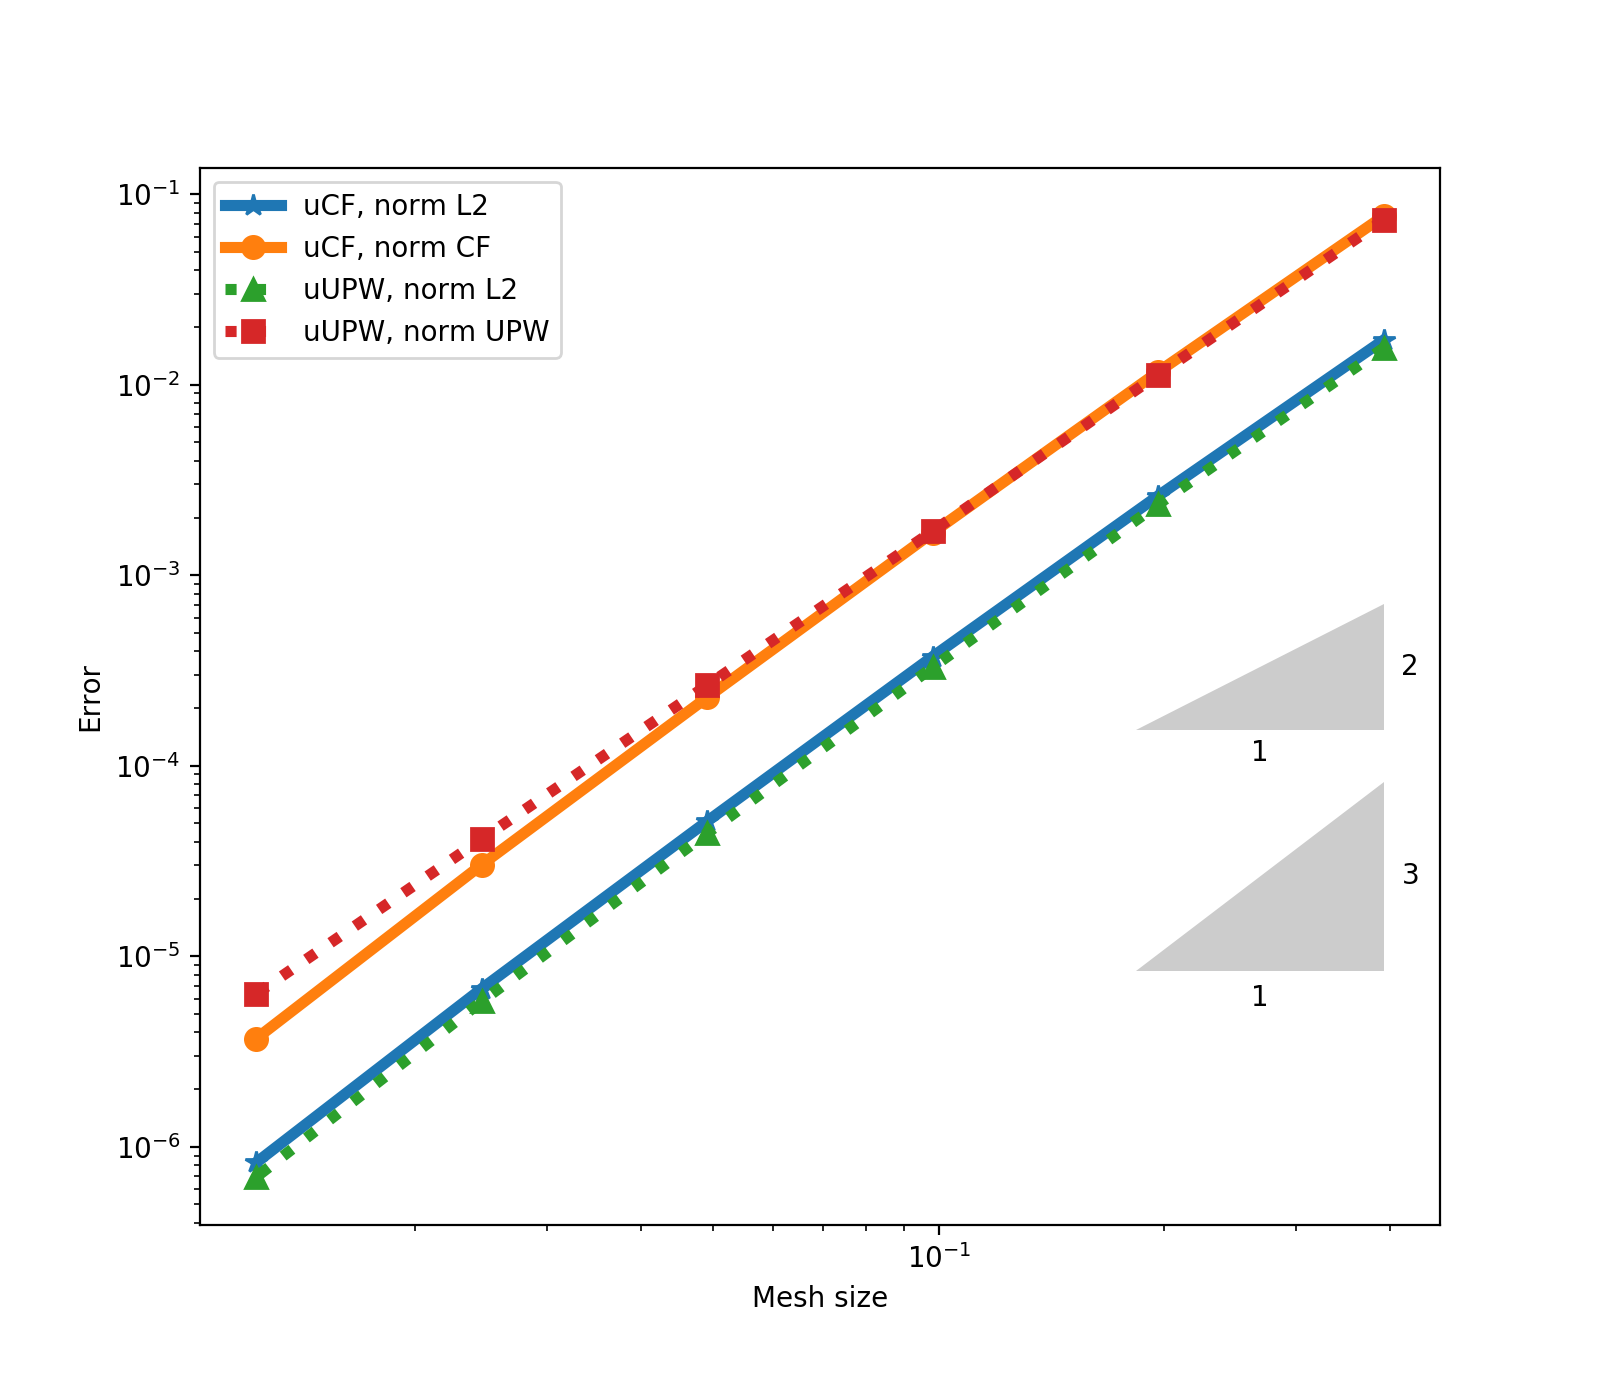
\includegraphics[scale=0.30]{img/Conveccion_Reaccion/errores_conveccion_reaccion_P2dc.png}
			\captionof{figure}{Errors in logarithmic scale.}
		\end{minipage}
		\end{frame}

	\section{Nontrivial examples}
		\begin{frame}{Properties of upwind $\mathbb{P}_0(\T_h)$ DG methods}
		Generalizing the upwind DG approximation and using $\mathbb{P}_0(\T_h)$ we have been able to develop approximations of several models that satisfy: 
		\vspace*{0.5cm}
			\begin{itemize}\itemsep1em
				\item Local mass conservation.
				\item Bound preserving.
				\item Energy stability.
			\end{itemize}
		\end{frame}

		\begin{frame}{Advective Cahn-Hilliard equation}
			
		\end{frame}

		\begin{frame}{Keller-Segel model}
			
		\end{frame}

		\begin{frame}{Phase-field tumor model}
			
		\end{frame}

\begin{frame}{References}
	\scriptsize 
	\vspace*{-0.25cm}
	\nocite*
	\bibliographystyle{apalike}
	\bibliography{references}
\end{frame}

\begin{frame}{}
	\centering
	\vspace*{1cm}
	{\Huge
		\emph{Thanks for your attention!}}
	
	\vspace*{0.5cm}
	
	\vspace*{1cm}
	\begin{acknowledgements}
		The speaker has been supported by a \textit{Graduate Scholarship funded by the University of Tennessee at Chattanooga}; by \textit{UCA FPU contract UCA/REC14VPCT/2020, Erasmus+ KA131 and travel grants funded by Universidad de Cádiz}.
	\end{acknowledgements}
\end{frame}